\documentclass[a4paper,12pt]{article}
\usepackage[utf8]{inputenc}

\usepackage[english,russian]{babel}
\usepackage[left=2cm,right=1cm,top=1cm,bottom=1cm]{geometry}
\usepackage{
	amsmath, amssymb, % math
	float, % for table captions
	hyperref, % fancy links
	listings, % sources
	graphicx, % pictures
	mathtools,xparse, % for norm, normL
	dutchcal, % lowercase mathcal font
	empheq, % boxed eqns
	titlesec, % subsectioning
	pdflscape, % portrait landscape (for large tables)
%	arydshln, % fancy lines for tables
	booktabs, % toprule, midrule, … for tables
	bm % bold for everything
}
\usepackage[dvipsnames]{xcolor} % fancy colors

\hypersetup{
	colorlinks,
	linkcolor={blue!60!black},
	citecolor={blue!60!black},
	urlcolor={blue!70!black}
}

\lstset{
	texcl,
	escapechar=`,
	escapebegin=\lst@commentstyle,
    basicstyle=\small\ttfamily\color{black},
    keywordstyle=\color{green!40!black},
    emphstyle=\bfseries\color{green!40!black},
    commentstyle=\itshape\color{purple!40!black},
    identifierstyle=\color{blue!30!black},
    showstringspaces=false,
    stringstyle=\color{orange},
    numbers=left,
    tabsize=2,
    breaklines=true,
    breakatwhitespace=true
}

% table captions
\restylefloat{table}
\let\oldtabular\tabular
\renewcommand{\tabular}{\footnotesize\oldtabular}

% roman numbering for sections
\renewcommand{\thesection}{\Roman{section}}
% paragraph subsectioning
\titleformat{\paragraph}
{\normalfont\normalsize\bfseries}{\theparagraph}{1em}{}
\titlespacing*{\paragraph}
{0pt}{3.25ex plus 1ex minus .2ex}{1.5ex plus .2ex}
\renewcommand{\theparagraph}{\thesubsubsection.\alph{paragraph}}
\setcounter{secnumdepth}{4}
\setcounter{tocdepth}{4} % table of contents   

% norms
\DeclarePairedDelimiter{\abs}{\lvert}{\rvert}
\DeclarePairedDelimiter{\norm}{\lVert}{\rVert}
\NewDocumentCommand{\normL}{ s O{} m }{%
	\IfBooleanTF{#1}{\norm*{#3}}{\norm[#2]{#3}}_{L_2(\Omega)}%
}

% differentials
\newcommand*\diff{\mathop{}\!\mathrm{d}}
\newcommand*\Diff[1]{\mathop{}\!\mathrm{d^#1}}

% span{…}, area, length
\DeclareMathOperator{\spn}{span}
\DeclareMathOperator{\area}{area \, of}
\DeclareMathOperator{\length}{length \, of}

% bold vectors
\newcommand{\vect}[1]{\boldsymbol{\mathbf{#1}}}

\begin{document}
    \begin{titlepage}
    \begin{center}
        Министерство образования и науки Российской Федерации\\
        Новосибирский государственный технический университет\\
        Кафедра прикладной математики
        \vfill
        \Large
        Курсовая работа\\ 
        по дисциплине «Уравнения математической физики»\\
        \Huge
        \textbf{Решение начально--краевых задач для уравнений гиперболического типа в двумерных областях с помощью связки МКЭ и МКР}
    \end{center}

    \vfill

    \begin{tabbing}
        Преподаватель \quad\= Персова М.\,Г.\kill
        Факультет     \> ПМИ\\
        Группа        \> ПМ\;33\\
        Студент       \> Жиляков А.\\
        Преподаватель \> Персова М.\,Г.\\
        Вариант       \> 7
    \end{tabbing}

    \vfill

    \begin{center}
        Новосибирск, 2016
    \end{center}
\end{titlepage} 
    \tableofcontents
    \thispagestyle{empty} % no page num. on table of contents
    \newpage
    \listoffigures
    \listoftables
	\thispagestyle{empty} % no page num. on table of contents
    \newpage
    \newgeometry{ % geometry for the rest pages
    	left=2cm,
    	right=1cm,
    	top=1cm,
    	bottom=1cm,
    	includefoot,
    	heightrounded
    }
    % main parts
    Исходные тексты программы доступны в репозитории:\\
\url{https://github.com/CATSPDEs}

Комплекс программ для численного решения уравнений в частных производных разработан с использованием \texttt{C++11} (\texttt{Visual Studio 2015}, компилятор \texttt{MSVC}).

Для аналитических вычислений (расчёта локальных матриц и векторов, производных временного базиса и т.\,д.), оформления таблиц, рисунков и анимаций полученных решений использовалась мощная система символьной арифметики \texttt{Mathematica 10.4}.

\section{Стационарная задача}
\label{stationary}

Пусть дано уравнение\footnote{
	Уравнение вида $u_t - \nabla \cdot (a \, \nabla u) + r(u) = 0$ называют \textbf{уравнением диффузии--реакции} (\textit{diffusion--reaction eqn}). Слагаемое с оператором Лапласа «отвечает» за диффузию (или теплопроводность), зависящее от решения $u$ слагаемое --- за реакцию среды. 
	
	Если уравнение содержит конвективное слагаемое $q(\nabla u)$, то уравнение называют \textbf{уравнением конвекции--диффузии} (\textit{convection--diffusion eqn}).
	
	Если решение не зависит от времени ($u_t \equiv 0$) --- т.\,е. мы имеем дело со стационарной проблемой --- и $r(u) = c \, u - f$, то задача сводится к \textbf{стационарному уравнению диффузии--реакции} (\textit{steady--state diffusion--reaction eqn})~(\ref{eqn}).
	
	По этим причинами мы называем входящие в~(\ref{eqn}) функции $a$ и $c$ коэффициентами диффузии и реакции соответственно.  
}
\begin{equation}
	\label{eqn}
	- \nabla \cdot (a \, \nabla u) + c \, u = f, \quad \vect{x} \in \Omega,
\end{equation}
с краевыми условиями
\begin{equation}
	\label{BCs}
	- \vect{\hat{n}} \cdot (a \, \nabla u) = \kappa \, (u - g_D) - g_N, \quad \vect{x} \in \partial \Omega,
\end{equation}
где $\vect{x} \coloneqq (x, \, y) \in \mathbb{R}^2$~--- аргумент, $a$, $c$, $f$, $\kappa$, $g_D$ и $g_N$~--- заданные $\mathbb{R}^2 \rightarrow \mathbb{R}$ функции, $\Omega \subset \mathbb{R}^2$~--- отрытая область с кусочно--гладкой границей $\partial \Omega$, $\vect{\hat{n}} \: : \: \mathbb{R}^2 \rightarrow \mathbb{R}^2$~--- нормированный вектор, нормальный к $\partial \Omega$ и направленный вне области. 

Нужно найти решение $u = u(\textbf{x})$, удовлетворяющее~(\ref{eqn}~--~\ref{BCs}).

\subsection{Вариационная постановка}
\label{Galerkin}

Аналитическое решение задачи~(\ref{stationary}) на практике доступно редко --- оно может быть найдено для «ограниченного» набора входных в (\ref{eqn}~--~\ref{BCs}) функций и «простых» областей. Подробно аналитические методы решения уравнений в частных производных рассмотрены в~\cite{PDEs}.

Мы рассмотрим методы численного решения задачи~(\ref{stationary}) (в этой секции --- методом конечных элементов (МКЭ), в следующей --- связкой МКЭ и метода конечных разностей (МКР) для нестационарной задачи). 

Предположим\footnote{
	Зачастую функция $u$ интерпретируется как температура плоской области $\Omega$. Известно, что температура пропорциональна скорости движения частиц в точке $\vect{x}$: $u(\vect{x}) \propto V(\vect{x})$, $u^2(\vect{x}) \propto V^2(\vect{x})$. Принимая во внимание конечность кинетической энергии, можно утверждать, что 
	$$
		\infty > \int_\Omega u^2(\vect{x}) \diff{\vect{x}} \eqqcolon \normL{u}^2.
	$$
	Стало быть, пространство Лебега --- подходящее место жительства для искомого решения.
}, что решение задачи~(\ref{stationary}) живёт в гильбертовом пространстве 
\begin{equation}
\label{V}
	\mathbb{V} \coloneqq \{ v = v(\vect{x}): \normL{v} + \normL{\nabla v} < \infty \}.
\end{equation}

Домножим (в смысле скалярного произведения в $L_2$) уравнение~(\ref{eqn}) на тестовую функцию~$v~\in~\mathbb{V}$:
\begin{subequations}
\label{multByTestFunc}
	\begin{align}
		\int_{\Omega} f \, v \diff{\vect{x}}  
		&= 
		\int_{\Omega} - \nabla \cdot (a \, \nabla u) \, v \diff{\vect{x}}  + 
		\int_{\Omega} c \, u \, v \diff{\vect{x}}  \\
		&= 
		\int_{\Omega} a \, \nabla u \cdot \nabla v \diff{\vect{x}}  -
		\int_{\partial \Omega} \vect{\hat{n}} \cdot (a \, \nabla u) \, v \diff{s} +
		\int_{\Omega} c \, u \, v \diff{\vect{x}}  \label{green} \\
		&= 
		\int_{\Omega} a \, \nabla u \cdot \nabla v \diff{\vect{x}}  +
		\int_{\partial \Omega} ( \kappa \, (u - g_D) - g_N ) \, v \diff{s} +
		\int_{\Omega} c \, u \, v \diff{\vect{x}} . \label{applyBCs}
	\end{align}
\end{subequations}
В~(\ref{green}) мы воспользовались теоремой Грина интегрирования по частям, в~(\ref{applyBCs}) --- краевыми условиями~(\ref{BCs}).

Перепишем уравнение~(\ref{multByTestFunc}) так, чтобы все слагаемые, зависящие от $u$, остались слева:
\begin{equation}
	\label{varForm}
	\mathbcal{a}(u, v) 
	\coloneqq
	\int_{\Omega} a \, \nabla u \cdot \nabla v \diff{\vect{x}}  + 
	\int_{\Omega} c \, u \, v \diff{\vect{x}}  +
	\int_{\partial \Omega} \kappa \, u \, v \diff{s}
	=
	\int_{\Omega} f \, v \diff{\vect{x}}  +
	\int_{\partial \Omega} ( \kappa \, g_D + g_N ) \, v \diff{s}
	\eqqcolon
	\mathbcal{l}(v).
\end{equation}
Здесь $\vect{\mathbcal{a}}$ суть билинейная форма и $\mathbcal{l}$ --- линейный функционал, определённые на $\mathbb{V}$.

Потребуем, чтобы равенство~(\ref{varForm}) выполнялось для всех тестовых функций $v \in \mathbb{V}$. Такая задача называется \textbf{слабой формой} (или \textbf{вариационной постановкой}, или \textbf{задачей Галёркина}) для исходной задачи~(\ref{stationary}):
\begin{empheq}[box=\fbox]{align}
	\label{weakForm}
	\begin{split}
		&\text{Найти пробную функцию } u \in \mathbb{V}, \text{ такую что равенство} \\
		&\mathbcal{a}(u, v) = \mathbcal{l}(v) \\
		&\text{справедливо для всех тестовых функций } v \in \mathbb{V}.
	\end{split}
\end{empheq}

Очевидно, что если $u$ есть решение задачи~(\ref{stationary}), то оно удовлетворяет задаче~(\ref{weakForm}). Обратное не так очевидно. Состоятельность --- существование и единственность решения --- задачи~(\ref{weakForm}) гарантируется при наложении некоторых ограничений на $\vect{\mathbcal{a}}$ и $\mathbcal{l}$ (теорема Лакса---Мильграма).

Доказательства состоятельности слабых форм некоторых задач типа~(\ref{stationary}) (задача Дирихле для уравнения Пуассона, задача Неймана для уравнения диффузии--реакции и т.д.) можно найти в~\cite[с.~192]{umea}. О задачах Галёркина и Ритца можно прочесть в~\cite{balandinFEM}.

В данной работе мы не будем останавливаться на аналитике и перейдём к тому, как грамотно запрограммировать и решить задачу~(\ref{weakForm}) на компьютере.

\subsection{Переход к конечномерному подпространству}
\label{chooseVh}

Пусть $\mathbb{V}_h := \spn \{ \phi_1, \phi_2, \dots, \phi_n \} \subset \mathbb{V}$ --- некоторое известное конечномерное подпространство, $n \coloneqq \dim \mathbb{V}_h$. Будем искать приближение $u_h(\textbf{x}) = \sum_{1}^{n} \xi_i \, \phi_i(x)$ к решению $u$ задачи~(\ref{weakForm}) в нём:
\begin{empheq}[box=\fbox]{align}
	\label{discreteWeakForm}
	\begin{split}
		&\text{Найти пробную функцию } u_h \in \mathbb{V}_h, \text{ такую что равенство} \\
		&\mathbcal{a}(u_h, v) = \mathbcal{l}(v) \\
		&\text{справедливо для всех тестовых функций } v \in \mathbb{V}_h.
	\end{split}
\end{empheq}

Очевидно, что определение функции $u_h$ эквивалентно нахождению её $n$ базисных коэффициентов (весов) $\xi_i$. Также очевидно, что требование «…справедливо для всех тестовых функций $v \in \mathbb{V}_h$» в~(\ref{discreteWeakForm}) эквивалентно требованию «…справедливо для $\phi_1, \, \phi_2, \, \dots, \, \phi_n$». Тогда задача~(\ref{discreteWeakForm}) эквивалентна решению СЛАУ
\begin{equation}
	\label{SLAE}
	\underbrace{(\vect{M} + \vect{S} + \vect{R})}_{\eqqcolon \vect{A}}
	\,
	\vect{\xi} 
	= 
	\overbrace{\vect{f} + \vect{r}}^{\eqqcolon \vect{b}},
\end{equation}
где $\vect{A}$ суть симметричная матрица системы, $\vect{b}$ --- вектор правой части, $\vect{\xi} \coloneqq (\xi_1, \, \xi_2, \, \dots, \, \xi_n)^T$ --- вектор неизвестных и
\begin{subequations}
\label{how2compute}
	\begin{align}
		\vect{M}_{i \, j} &\coloneqq \int_{\Omega} c \, \phi_i \, \phi_j \diff{\vect{x}} , \label{massEl} \\
		\vect{S}_{i \, j} &\coloneqq \int_{\Omega} a \, \nabla \phi_i \cdot \nabla \phi_j \diff{\vect{x}} , \label{stiffnessEl} \\
		\vect{R}_{i \, j} &\coloneqq \int_{\partial \Omega} \kappa \, \phi_i \, \phi_j \diff{s}, \label{RobinMatrixEl} \\
		\vect{f}_i        &\coloneqq \int_{\Omega} f \, \phi_i \diff{\vect{x}} , \label{loadEl} \\
		\vect{r}_i        &\coloneqq \int_{\partial \Omega} ( \kappa \, g_D + g_N ) \, \phi_i \diff{\vect{x}} . \label{RobinVectorEl}
	\end{align}
\end{subequations}

По историческим причинам матрицу~\vect{M} называют \textbf{матрицей масс} (\textit{mass matrix}), матрицу~\vect{S}~--- \textbf{матрицей жёсткости} (\textit{stiffness matrix}) и вектор~\vect{f}~--- \textbf{вектором нагрузки} (\textit{load vector}).

Матрица~\vect{R} и вектор~\vect{r} не имеют устоявшихся названий, но мы здесь будем обозначать их \textbf{матрицей и вектором Робина} соответственно. Причиной этому служит тот факт, что в них дают вклады интегралы по границе, интегранды которых определяются краевым условием~(\ref{BCs}), которое часто называют условием Робина (или обобщённым условием Неймана, или просто краевым условием 3--го типа).

Таким образом, решение задачи~(\ref{discreteWeakForm}) сводится к
\begin{enumerate}
	\item выбору базиса подпространства~$\mathbb{V}_h$, 
	\item сборке (в МКЭ принято слово \textit{ассемблирование}) матрицы~\vect{A} и вектора~\vect{b} системы~(\ref{SLAE})
	\item и её решению. 
\end{enumerate}

\subsection{Выбор конкретного конечномерного подпространства и дискретизация расчётной области}
\label{workOnDiscreteMesh}

Наиболее распространённые дискретные области, которые используются в МКЭ для двумерных задач, --- это области, разбитые на конечное множество треугольников (триангуляции) или прямоугольников.

Триангуляции --- наиболее гибкий инструмент в том смысле, во--первых, что с помощью них можно очень эффективно приближать криволинейные границы, а значит, решать задачи на практически любых расчётных областях. Во--вторых, существует множество уже готовых и эффективных алгоритмов построения «качественных»\footnote{
	Здесь под качеством понимается «мера близости» треугольников к правильным. Оказывается, наличие «плоских» треугольников (их называют \textit{вырожденными}) оказывает влияние на качество МКЭ--решения. Но об этом позже. 
} сеток (алгоритмы Делоне). \\
В этой работе мы будем рассматривать только треугольные сетки.

\begin{figure}[!h]
	\minipage{0.45\textwidth}
	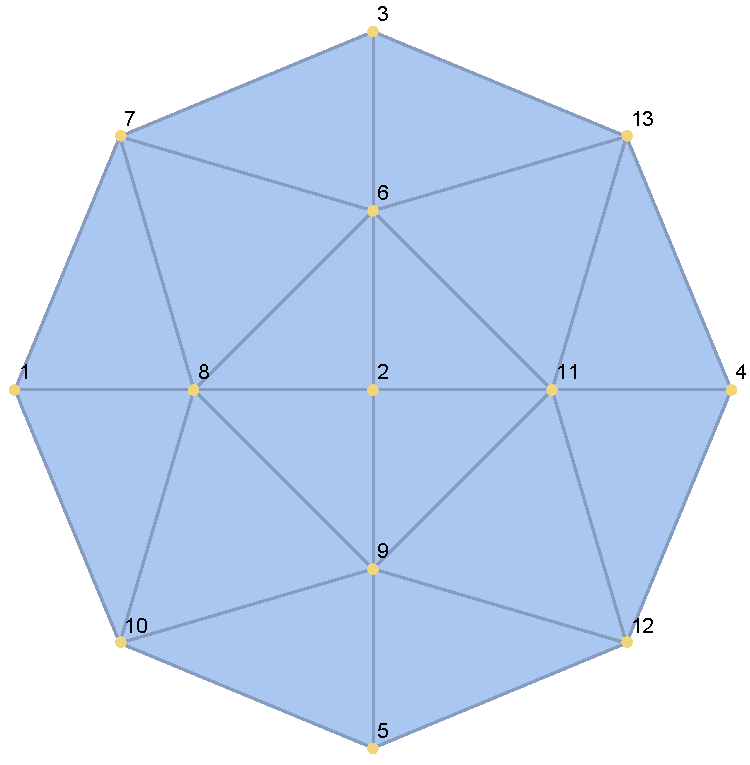
\includegraphics[width=\linewidth]{img/typicalMesh.pdf}
	\caption{Типичная триангуляция диска}\label{fig:typicalMesh}
	\endminipage\hfill
	\minipage{0.45\textwidth}
	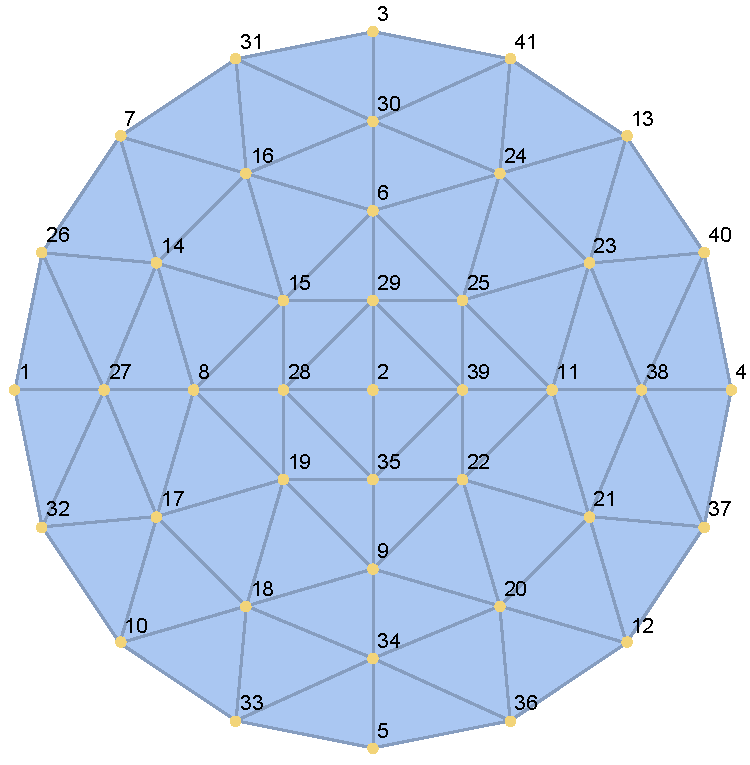
\includegraphics[width=\linewidth]{img/typicalMeshRefined.pdf}
	\caption{Измельчённая триангуляция диска. Обратите внимание, что кривизна границы с измельчением учитывается}\label{fig:typicalMeshRefined}
	\endminipage
\end{figure}

\begin{figure}[!h]
	\centering
	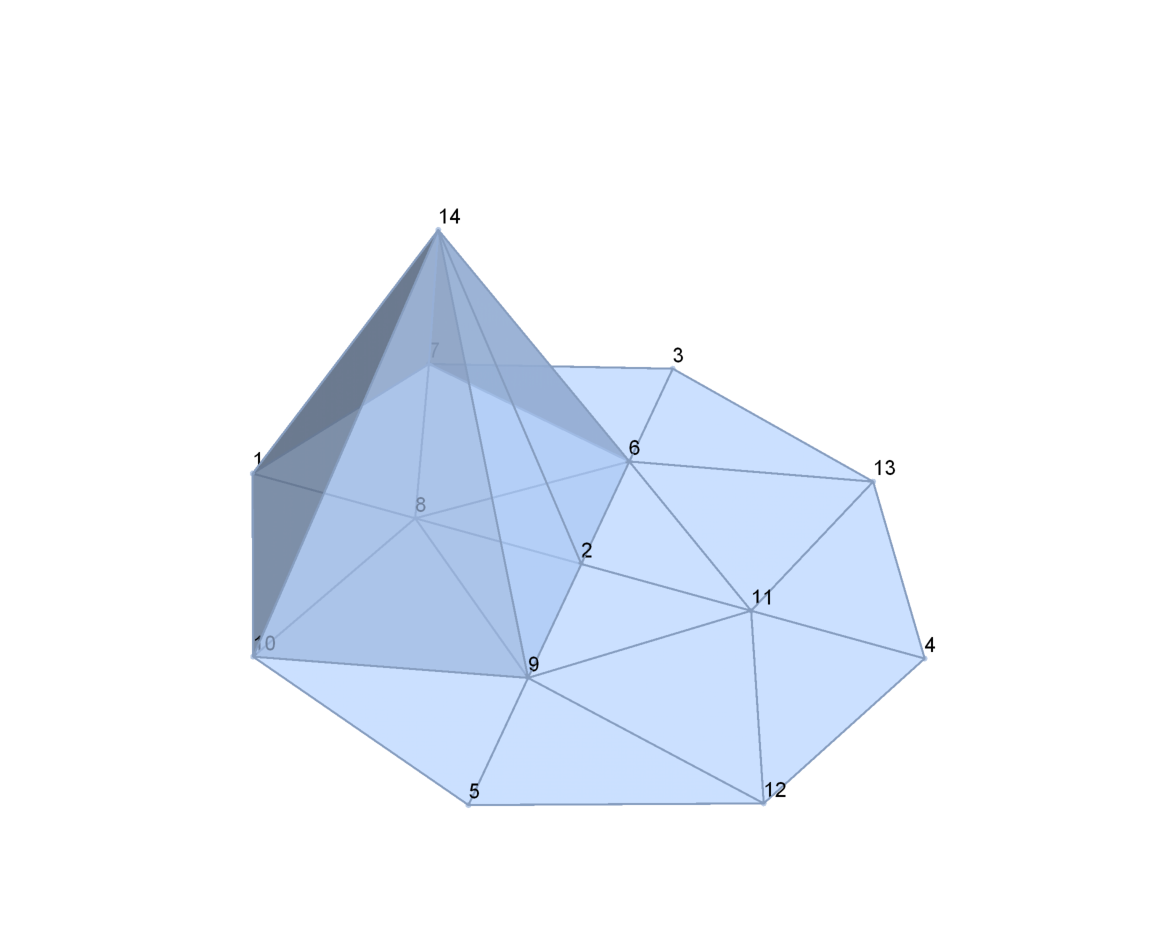
\includegraphics[width=0.8\linewidth]{img/typicalBasisFunc.pdf}
	\caption{Базисная функция $\phi_8$, определённая на сетке рис.~\ref{fig:typicalMesh}}
	\label{fig:typicalBasisFunc}
\end{figure}

Пусть $\Omega_h$ есть триангуляция области $\Omega$ --- множество вершин и элементов (треугольников). При этом каждый треугольник даёт в пересечении с другим треугольником либо пустое множество, либо вершину, либо ребро --- иными словами, триангуляция не может иметь «висячих» вершин. Очевидным требованием является сходимость меры $\Omega_{h / k}$ к мере $\Omega$ при $k \rightarrow \infty$. \\
Для триангуляций, вообще говоря, придумано целое множество абстракций для представления в компьютере. Более подробно мы обсудим этот вопрос позже, когда станут ясны все требования к нашей сетке.

Возьмём в качестве пространства $\mathbb{V}_h$ пространство всех непрерывных и линейных на каждом треугольнике функций, определённых на $\Omega_h$:
\begin{align}
	\mathbb{V}_h &= C^0(\Omega) \cap \{ v : v|_\Delta \in P_1(\Delta) \text{ для всех треугольников } \Delta \in \Omega_h \}, \label{Vh} \\
	P_1(\Delta) & \coloneqq \{ v : v(x, \, y) = c_1 \, x + c_2 \, y + c_3, \: (x, \, y) \in \Delta \} \label{p1Space}
\end{align}

В качестве базиса $\mathbb{V}_h$ выберем \textit{вершинный} базис (см. рис.~\ref{fig:typicalBasisFunc}):
\begin{align}
	\label{nodalBasis}
	\phi_i(\vect{x}_j) = \delta_{i \, j} \text{ для всех вершин } \vect{x_j} \text{ триангуляции } \Omega_h,
\end{align}
т.\,е. $i$--я функция базиса принимает единицу в $i$--й вершине и ноль иначе. 

В таком выборе базиса есть, как минимум, четыре преимущества:
\begin{enumerate}
	\item простота интерпретации базисных коэффициентов --- $u_h(\vect{x}_i) = \xi_i$,
	\item (вытекает из первого пункта) простота построения интерполяции $\pi_1 g(\vect{x}) \coloneqq \sum_1^n g(\vect{x}_i) \, \phi_i(\vect{x})$ любой известной функции $g$. Это полезно для расчёта квадратур, входящих в систему~(\ref{SLAE}),
	\item финитность базисных функций и, как следствие, \textbf{разреженность матрицы $\vect{A}$} и 
	\item элегантность алгоритма ассемблирования системы~(\ref{SLAE}) (подробно рассмотрим в разделе~(\ref{assembly})).
\end{enumerate} 

Третий пункт особенно важен, так как он позволяет решать задачи, приводящие к огромным СЛАУ, пользуясь ограниченной памятью компьютера.

\subsection{Учёт краевых условий}

Задание граничных условий~(\ref{BCs}) в виде тройки функций~$(\kappa, \, g_D, \, g_N)$ удобно тем, что оно единообразно описывает все три классических типа краевых условий: Дирихле, Неймана и Робина.

Пусть $\Gamma_D$, $\Gamma_N$ и $\Gamma_R \subset \partial \Omega$ суть не пересекающиеся части границы, в объединении дающие $\partial \Omega$, на которых заданы краевые условия Дирихле, Неймана и Робина соответственно. Задания условий на поток через границу очевидны; для условий Неймана достаточно положить $\kappa(\Gamma_N) = \{ 0 \}$, для условий Робина --- $g_D(\Gamma_R) = \{ 0 \}$:
\begin{align*}
\vect{\hat{n}} \cdot (a \, \nabla u) = g_N,               &\quad \vect{x} \in \Gamma_N, \\
\vect{\hat{n}} \cdot (a \, \nabla u) + \kappa \, u = g_N, &\quad \vect{x} \in \Gamma_R.
\end{align*}

Краевые условия Дирихле $u = g_D, \: \vect{x} \in \Gamma_D$ нельзя учесть явно с использованием~(\ref{BCs}), однако их можно аппроксимировать условиями Робина. Перепишем~(\ref{BCs}) в виде
$$
u - g_D = \frac{ g_N - \vect{\hat{n}} \cdot (a \, \nabla u) }{ \kappa }.
$$

Положив $g_N(\Gamma_D) = \{ 0 \}$ и $\kappa(\Gamma_D)$ достаточно большим (скажем, порядка $10^{50}$), получим $u - g_D \simeq 0$ --- фактически равенство в конечной арифметике компьютера.

С практической точки зрения такой учёт условий Дирихле означает внесение возмущений в $\vect{A}$ и $\vect{b}$ --- взгляните на элементы матрицы и вектора Робина~(\ref{RobinMatrixEl}) и~(\ref{RobinVectorEl}). \\
В них дают вклад интегралы, в интегранды которых входит $\kappa = 10^{50}$. 

Существует два распространённых способа учёта условий Дирихле:
\begin{enumerate}
	\item для всех $\vect{x}_j \in \Gamma_D$ обнулить $j$--ю строчку матрицы~$\vect{A}$, установить $\vect{A}_{j \, j} = 1$ и $\vect{b}_{j} = g_D(\vect{x}_j)$,
	\item для всех $\vect{x}_j \in \Gamma_D$ положить $\vect{b}_{j} = g_D(\vect{x}_j)$ и домножить $\vect{b}_{j}$ и $\vect{A}_{j \, j}$ на большое число (скажем, на $10^{50}$).
\end{enumerate}

Первый подход фактически заменяет $j$--е уравнение системы~(\ref{SLAE}) на уравнение $\xi_j =  g_D(\vect{x}_j)$, второй --- на уравнение $\xi_j \simeq g_D(\vect{x}_j)$, нивелируя вклад остальных слагаемых уравнения\footnote{
	В МКЭ в качестве базиса выбирают \textit{вершинный базис}, т.\,е. такой, что $\phi_i(\vect{x}_j) = \delta_{i \, j}$ (символ Кронекера). Поэтому вес $\xi_j$ суть значение функции $u_h$ в $j$--м узле. 	
}.

По своей сути наш подход совпадает со вторым, однако у него есть приятный бонус: нет никакой необходимости заботиться об учёте условий Дирихле отдельно, изменяя матрицу и вектор системы --- \textit{учёт условий всех типов происходит единообразно}.

Первый подход наиболее «честный» в том смысле, что решение ищется в «правильном» пространстве $\mathbb{V}_{h, \, D} := \mathbb{V}_h \cap \{ v : v(\vect{x}) = g_D(\vect{x}) \text{ для всех } \vect{x} \in \Gamma_{D} \}$. Однако такой подход нарушает симметричность матрицы $\vect{A}$. Как следствие, приходится либо симметризовывать матрицу, либо использовать несимметричный формат хранения, увеличивая расходы на память компьютера.

В данной работе мы не будем использовать первый подход.

\subsection{Ассемблирование СЛАУ}
\label{assembly}

\subsubsection{Вклады квадратур по элементам}
\label{elementAssembly}

В сердце МК\textbf{Э} --- ассемблирование матрицы~\vect{A} и вектора~\vect{b}, которое очень удобно и быстро осуществлять при обходе \textbf{элементов} (в нашем случае --- треугольников) сетки $\Omega_h$. Отсюда первое требование к абстракции для сетки --- \textbf{элементы необходимо хранить явно}.

Рассмотрим процесс сборки на примере $\Omega_h$, представленной на рис.~\ref{fig:assemblyMesh}.

\begin{figure}[!h]
	\centering
	\resizebox{0.8\textwidth}{!}{\input{img/assemblyMesh.pdf_tex}}
	\caption{{\color{Plum} Глобальная нумерация узлов}, {\color{OliveGreen} локальная нумерация узлов} и глобальная нумерация элементов, задаваемые абстракциями $\vect{\mathcal{V}}$ и $\vect{\mathcal{T}}$}
	\label{fig:assemblyMesh}
\end{figure}

Триангуляция\footnote{
	Здесь и далее для упрощения нотаций мы будем использовать верхний индекс со скобками $(i)$ для указания того, что объект имеет отношение к $i$--му элементу сетки $\Delta^{(i)}$.
} $\Omega_h = \cup_1^3 \Delta^{(i)}$ (рис.~\ref{fig:assemblyMesh}) может быть представлена списком вершин $\vect{\mathcal{V}}$ и «треугольников» (указатели на элементы $\vect{\mathcal{V}}$) $\vect{\mathcal{T}}$:
\begin{align*}
	\vect{\mathcal{V}} &\coloneqq \langle \quad
		( \frac{1}{2}, \, \frac{\sqrt{2}}{2} ), \,
		( -\frac{1}{2}, \, \frac{\sqrt{2}}{2} ), \,
		( \frac{3}{2}, \, \frac{\sqrt{2}}{2} ), \,
		(1, \, 0), \,
		(0, \, 0)
	\quad \rangle, \\
	\vect{\mathcal{T}} &\coloneqq \langle \quad
	( 5, \, 4, \, 1 ), \,
	( 1, \, 4, \, 3 ), \,
	( 2, \, 5, \, 1 )
	\quad \rangle.
\end{align*}

Заметим, что каждый элемент $\vect{\mathcal{T}}_i$ определяет отображение $\vect{\mathcal{n}}^{(i)} \: : \: \{ 1, \, 2, \, 3 \} \rightarrow \{ \vect{\mathcal{T}}_{i \, 1}, \, \vect{\mathcal{T}}_{i \, 2}, \, \vect{\mathcal{T}}_{i \, 3} \}$ {\color{OliveGreen} локальной} нумерации вершин на {\color{Plum} глобальную}. \\
Например, для первого треугольника $\Delta^{(1)}$ соответствие между {\color{OliveGreen} локальной} и {\color{Plum} глобальную} нумерацией определяется $\vect{\mathcal{n}}^{(1)}({\color{OliveGreen} 1}) = {\color{Plum} 5}$, $\vect{\mathcal{n}}^{(1)}({\color{OliveGreen} 2}) = {\color{Plum} 4}$ и $\vect{\mathcal{n}}^{(1)}({\color{OliveGreen} 3}) = {\color{Plum} 1}$ (см. рис.~\ref{fig:assemblyMesh}).

Вершины $\vect{x}^{(i)}_1 \coloneqq (x^{(i)}_1, \, y^{(i)}_1)$, $\vect{x}^{(i)}_2 \coloneqq (x^{(i)}_2, \, y^{(i)}_2)$ и $\vect{x}^{(i)}_3 \coloneqq (x^{(i)}_3, \, y^{(i)}_3)$, образующие треугольник $\Delta^{(i)}$, могут быть получены так:
$$
	\vect{x}^{(i)}_j = \vect{\mathcal{V}}_{\mathcal{n}_i(j)}.
$$
Продемонстрируем ассемблирование на примере матрицы масс:
\begin{align}
\label{massMatrixAssembly}
	\begin{split}
		\vect{M} =
		& 
		\int_{\Omega_h} c 
			\begin{bmatrix}
				\phi_1 \, \phi_1 & \phi_1 \, \phi_2 & \phi_1 \, \phi_3 & \phi_1 \, \phi_4 & \phi_1 \, \phi_5 \\
				                 & \phi_2 \, \phi_2 & \phi_2 \, \phi_3 & \phi_2 \, \phi_4 & \phi_2 \, \phi_5 \\
				                 &                  & \phi_3 \, \phi_3 & \phi_3 \, \phi_4 & \phi_3 \, \phi_5 \\
				                 &                  &                  & \phi_4 \, \phi_4 & \phi_4 \, \phi_5 \\	
				\text{сим.}	     &                  &                  &                  & \phi_5 \, \phi_5			               
			\end{bmatrix}
		\diff{\vect{x}} 
		= \\
		&
		\int_{\Delta_1} c 
		\begin{bmatrix}
			\phi_1 \, \phi_1 & 0 & 0 & \phi_1 \, \phi_4 & \phi_1 \, \phi_5 \\
			&0&0&0&0 \\
			&&0&0&0 \\
			&&& \phi_4 \, \phi_4 & \phi_4 \, \phi_5 \\	
			\text{сим.}	&&&& \phi_5 \, \phi_5			               
		\end{bmatrix}
		\diff{\vect{x}} 
		+
		\int_{\Delta_2} c 
		\begin{bmatrix}
			\phi_1 \, \phi_1 & 0 & \phi_1 \, \phi_3 & \phi_1 \, \phi_4 & 0 \\
			&0&0&0&0 \\
			&& \phi_3 \, \phi_3 & \phi_3 \, \phi_4 & 0 \\
			&&& \phi_4 \, \phi_4 & 0 \\	
			\text{сим.} &&&& 0			               
		\end{bmatrix}
		\diff{\vect{x}}
		+ \\
		&
		\int_{\Delta_3} c 
		\begin{bmatrix}
			\phi_1 \, \phi_1 & \phi_1 \, \phi_2 & 0 & 0 & \phi_1 \, \phi_5 \\
			& \phi_2 \, \phi_2 & 0 & 0 & \phi_2 \, \phi_5 \\
			&&0&0&0 \\
			&&&0&0 \\
			\text{сим.} &&&& \phi_5 \, \phi_5			               
		\end{bmatrix}
		\diff{\vect{x}}
	\end{split}
\end{align}
В~(\ref{massMatrixAssembly}) мы воспользовались аддитивностью интеграла и финитностью базисных функций --- из построения базиса очевидно, что вклад в матрицу на треугольнике $\Delta^{(i)}$ дадут лишь три базисные функции, принимающие единицу в образующих его узлах (cм. рис.~\ref{fig:localBasis}).

На практике на каждом элементе $\Delta^{(i)}$ считается \textbf{локальная матрица} размерности $3 \times 3$
\begin{equation}
\label{localMassMatrix}
	\vect{\hat{M}}^{(i)} 
	=
	\int_{\Delta^{(i)}} c 
	\begin{bmatrix}
		\hat{\phi}^{(i)}_1 \, \hat{\phi}^{(i)}_1 & \hat{\phi}^{(i)}_1 \, \hat{\phi}^{(i)}_2 & \hat{\phi}^{(i)}_1 \, \hat{\phi}^{(i)}_3 \\
		& \hat{\phi}^{(i)}_2 \, \hat{\phi}^{(i)}_2 & \hat{\phi}^{(i)}_2 \, \hat{\phi}^{(i)}_3 \\
		\text{cим.} && \hat{\phi}^{(i)}_3 \, \hat{\phi}^{(i)}_3		               
	\end{bmatrix}
	\diff{\vect{x}},
\end{equation}
где $\hat{\phi}^{(i)}_j \coloneqq \phi_{\vect{\mathcal{n}}^{(i)}(j)}|_{\Delta^{(i)}}$ --- \textbf{локальная базисная функция} (см. рис.~\ref{fig:localBasis}); затем вносится вклад в матрицу системы $\vect{A}_{ \vect{\mathcal{n}}^{(i)}(j) \, \vect{\mathcal{n}}^{(i)}(k) } = \vect{A}_{ \vect{\mathcal{n}}^{(i)}(j) \, \vect{\mathcal{n}}^{(i)}(k) } + \vect{\hat{M}}_{j \, k}, \quad j = 1, \, 2, \, 3, \quad k = j, \, \dots, \, 3$ и осуществляется переход к следующему элементу $\Delta_{i+1}$.

Формулы для локальных базисных функций легко получить из определения~(\ref{nodalBasis}), записанного в матричном виде. $\hat{\phi}^{(i)}_j(x, \, y) = c^{(i)}_{j\,1} \, x + c^{(i)}_{j\,2} \, y + c^{(i)}_{j\,3}$ и 
\begin{equation}
\label{basisCoef}
	\underbrace{
		\begin{bmatrix}
			c^{(i)}_{1\,1} & c^{(i)}_{1\,2} & c^{(i)}_{1\,3} \\
			c^{(i)}_{2\,1} & c^{(i)}_{2\,2} & c^{(i)}_{2\,3} \\
			c^{(i)}_{3\,1} & c^{(i)}_{3\,2} & c^{(i)}_{3\,3}               
		\end{bmatrix}
	}_{\eqqcolon \vect{C}^{(i)}}
	\begin{bmatrix}
		x^{(i)}_1 & x^{(i)}_2 & x^{(i)}_3 \\
		y^{(i)}_1 & y^{(i)}_2 & y^{(i)}_3 \\
		1 & 1 & 1               
	\end{bmatrix}
	=
	\begin{bmatrix}
		1 & 0 & 0 \\
		0 & 1 & 0 \\
		0 & 0 & 1               
	\end{bmatrix},
\end{equation}
поэтому $\hat{\phi}^{(i)}_j = (\vect{C}^{(i)})^{-1}_{\cdot \, j} \cdot (x, \, y, \, 1)$.

Коэффициент реакции $c(\vect{x})$ может быть, вообще говоря, произвольной функцией. Поэтому для расчёта квадратур в~(\ref{localMassMatrix}) удобно заменить его линейной (или квадратичной) интерполяцией
\begin{subequations}
\label{interpolation}
	\begin{align}
		c|_{\Delta^{(i)}} \simeq 
		\pi_1 c^{(i)}(\vect{x}) & \coloneqq \sum_{j=1}^3 c(\vect{x}^{(i)}_j) \, \hat{\phi}^{(i)}_j(\vect{x}) \text{ или } \\
		\pi_2 c^{(i)}(\vect{x}) & \coloneqq \sum_{j=1}^6 c(\vect{x}^{(i)}_j) \, \hat{\psi}^{(i)}_j(\vect{x})
	\end{align}
\end{subequations}
где $\hat{\psi}^{(i)}_1$, $\hat{\psi}^{(i)}_2$, \dots, $\hat{\psi}^{(i)}_6$ --- квадратичные базисные функции (см. рис.~\ref{fig:localQuadBasis}), принимающие единицы на вершинах треугольника $\Delta^{(i)}$ и серединах его рёбер 
\begin{equation}
	\vect{x}^{(i)}_4 \coloneqq \frac{\vect{x}^{(i)}_2 + \vect{x}^{(i)}_3}{2},
	\quad
	\vect{x}^{(i)}_5 \coloneqq \frac{\vect{x}^{(i)}_1 + \vect{x}^{(i)}_3}{2},
	\quad
	\vect{x}^{(i)}_6 \coloneqq \frac{\vect{x}^{(i)}_1 + \vect{x}^{(i)}_2}{2}.
\end{equation}
Формулы для квадратичного базиса могут быть получены аналогично~(\ref{basisCoef}). Более того, можно заметить, что локальные квадратичные базисные функции можно выразить через произведения локальных линейных базисных функций.

Очевидно, что 	
\begin{align}
	c|_{\Delta^{(i)}} &= \pi_1 c^{(i)}(\vect{x}), \text{ если } c|_{\Delta^{(i)}} \in P_1(\Delta^{(i)}), \\
	c|_{\Delta^{(i)}} &= \pi_2 c^{(i)}(\vect{x}), \text{ если } c|_{\Delta^{(i)}} \in P_2(\Delta^{(i)}),
\end{align}
где $P_2(\Delta^{(i)})$ (аналогично $P_1(\Delta^{(i)})$, определённое в~(\ref{p1Space})) есть пространство полиномов 2-й степени, определённых на $i$--м элементе: 
\begin{align}
	P_2(\Delta^{(i)}) & \coloneqq \{ v : v(x, \, y) = c_1 \, x^2 + c_2 \, y^2 + c_3 \, x \, y + c_4 \, x + c_5 \, y + c_6, \: (x, \, y) \in \Delta^{(i)} \}, \\
	P_1(\Delta^{(i)}) & \subset P_2(\Delta^{(i)}).
\end{align}
Если же $c(\vect{x})$ не является полиномом, то с дроблением сетки интерполяция~(\ref{interpolation}) будет всё лучше его аппроксимировать.

\begin{figure}[!h]
	\minipage{0.45\textwidth}
	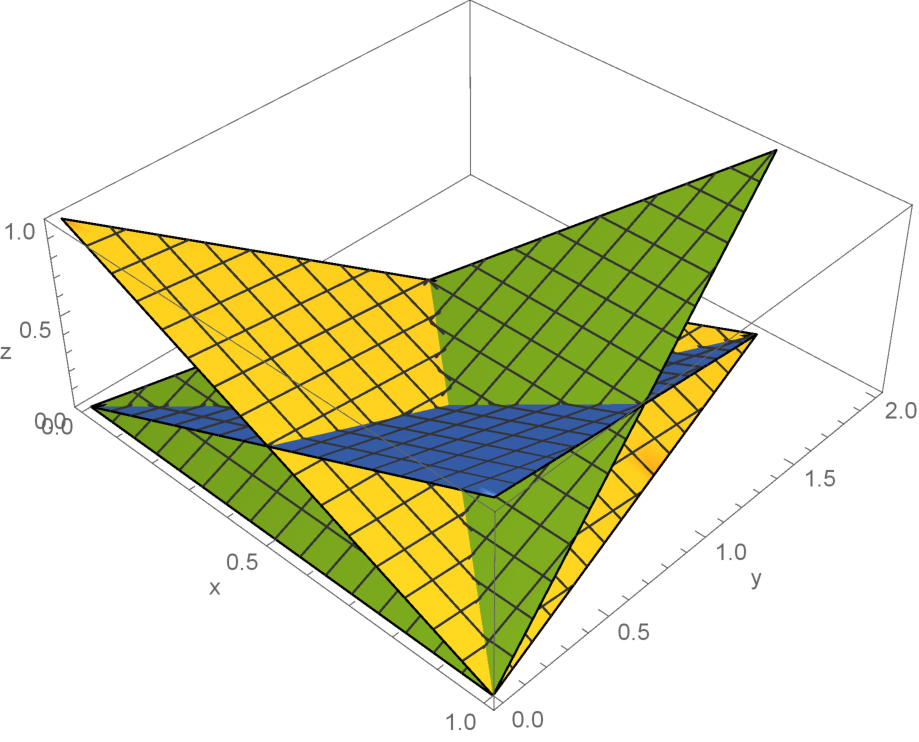
\includegraphics[width=\linewidth]{img/localBasis.pdf}
	\caption{Локальные базисные функции $\hat{\phi}^{(i)}_1$, $\hat{\phi}^{(i)}_2$ и $\hat{\phi}^{(i)}_3$, линейные на $i$-м элементе}\label{fig:localBasis}
	\endminipage\hfill
	\minipage{0.45\textwidth}
	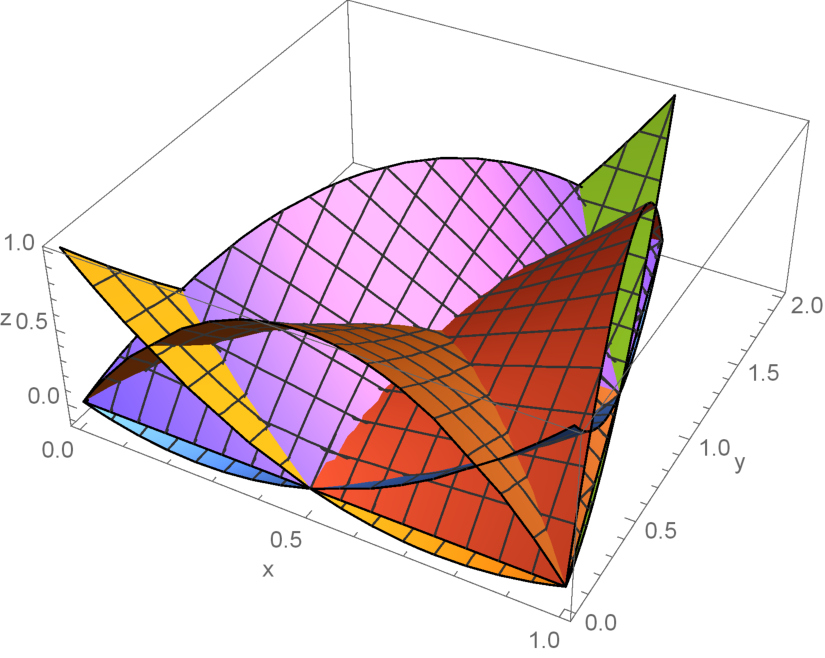
\includegraphics[width=\linewidth]{img/localQuadBasis.pdf}
	\caption{Локальные базисные функции $\hat{\psi}^{(i)}_1$, $\hat{\psi}^{(i)}_2$, \dots, $\hat{\psi}^{(i)}_6$, квадратичные на $i$-м элементе}\label{fig:localQuadBasis}
	\endminipage
\end{figure}

С учётом интерполяции~(\ref{interpolation}) и сказанного выше, вычисление квадратур для~(\ref{localMassMatrix}) сводится к вычислению интегралов типа
\begin{equation}
	\int_{\Delta^{(i)}} (\hat{\phi}^{(i)}_1(\vect{x}))^m \, (\hat{\phi}^{(i)}_2(\vect{x}))^l \, (\hat{\phi}^{(i)}_3(\vect{x}))^k \diff{\vect{x}},
\end{equation} 
вид которых известен (или может быть быстро посчитан, например, в системе \texttt{Mathematica}).

Сборка матрицы $\vect{S}$ и вектора $\vect{f}$ абсолютно аналогична, поэтому выкладки мы приводить не будем. \\
В секции~(\ref{localMatricesAndVectors}) приведены формулы для расчёта всех локальных матриц и векторов~(\ref{how2compute}), необходимых для сборки системы.

\subsubsection{Вклады квадратур по границе}
\label{boundaryAssembly}

Для того, чтобы ассемблировать вклады матрицы и вектора Робина, необходимо иметь доступ к границе $\Omega_h$. \textbf{Это второе требование к абстракции для нашей триангуляции}.

В принципе, можно было бы хранить список граничных «рёбер» --- список пар указателей на вершины в списке $\vect{\mathcal{V}}$ (подобно тому, как мы поступили с абстракцией для элементов $\vect{\mathcal{T}}$). \\
Однако мы откажемся от такого подхода по причинам, изложенным ниже.

\paragraph{Измельчение сетки и связанные с этим требования к абстракции для триангуляции}

Для уточнения решения часто необходимо измельчить сетку $\Omega_h$ --- решить задачу на более точной триангуляции $\Omega_\frac{h}{2}$. При этом дробиться могут не обязательно все\footnote{
	Примером может служить \textbf{адаптивный МКЭ} (\textit{adaptive FEM}). По окончании решения используется апостериорная оценка ошибки (основанная на скачках в градиентах полученного решения $u_h$), на основании которой конечное количество треугольников измельчается и решение пересчитывается.\\
	Об адаптивном МКЭ можно прочесть в~\cite[c.~97]{umea}.
} элементы $\Delta^{(i)}$.

Поэтому третье требование к абстракции --- возможность измельчать исходную сетку $\Omega_h$.

Добавление элементов (а значит, и новых узлов) приводит к появлению «висячих» вершин (мы обсудили это в секции~\ref{workOnDiscreteMesh}), нарушающих структуру триангуляции.

Чтобы избежать этой проблемы, удобно иметь доступ к $0 \le k \le 3$ смежным треугольникам («соседям») $\Delta^{(j)}$ текущего треугольника $\Delta^{(i)}$.\\ Для этого введём новую абстракцию $\vect{\mathcal{N}}$, элемент $\vect{\mathcal{N}}_i$ которой содержит тройку указателей на элементы $\vect{\mathcal{T}}$, являющиеся соседями элемента $\Delta^{(i)}$, описываемого $i$--м элементом абстракции $\vect{\mathcal{T}}$. Для сетки рис.~\ref{fig:assemblyMesh} описанная структура будет иметь вид:
\begin{subequations}
	\label{nodesAndNeighbors}
	\begin{align}
		\vect{\mathcal{V}} &\coloneqq \langle \quad
		( \frac{1}{2}, \, \frac{\sqrt{2}}{2} ), \,
		( -\frac{1}{2}, \, \frac{\sqrt{2}}{2} ), \,
		( \frac{3}{2}, \, \frac{\sqrt{2}}{2} ), \,
		(1, \, 0), \,
		(0, \, 0)
		\quad \rangle, \\
		\vect{\mathcal{T}} &\coloneqq \langle \quad
		( 5, \, 4, \, 1 ), \,
		( 1, \, 4, \, 3 ), \,
		( 2, \, 5, \, 1 )
		\quad \rangle, \\
		\vect{\mathcal{N}} &\coloneqq \langle \quad
		( 2, \, 3, \, -1 ), \,
		( -1, \, -1, \, 1 ), \,
		( 1, \, -1, \, -1 )
		\quad \rangle.
	\end{align}
\end{subequations}

Обратите внимание, что если ребро треугольника $\vect{\mathcal{T}}_i$ напротив $k$--го узла $\vect{\mathcal{V}}_{\vect{\mathcal{n}}_i(k)}$ является частью границы (т.\,е. у треугольника нет соседа по этому ребру), то $\vect{\mathcal{N}}_{i\,k} = -1$. \\
Например, как видно из рис.~\ref{fig:assemblyMesh} и~(\ref{nodesAndNeighbors}), 3--е ребро (ребро напротив 3--й вершины) 1--го треугольника является частью границы. Поэтому $\vect{\mathcal{N}}_{1\,3} = -1$.

Условимся, что узлы в тройках $\vect{\mathcal{T}}_{i}$ занумерованы так, что обход вершин $i$-го треугольника ведётся \textbf{против часовой стрелки} (справедливо для нашего примера~(\ref{nodesAndNeighbors})). Это удобно, потому что интегралы по границе в~(\ref{multByTestFunc}) берутся при её обходе против часовой стрелки.\\
Таким образом, не будет путаницы при учёте знака в процессе сборки вкладов матрицы~(\ref{RobinMatrixEl}) и вектора Робина~(\ref{RobinVectorEl}) в СЛАУ~(\ref{SLAE}).

Структура $\langle \vect{\mathcal{V}}, \, \vect{\mathcal{T}}, \, \vect{\mathcal{N}}\rangle$ называется «\textbf{узлы и треугольники}» (см.~\cite[с.~14]{delaunay}).

При использовании данной структуры все перечисленные выше требования к абстракции для триангуляции выполняются. Как было замечено в начале раздела~\ref{boundaryAssembly}, мы освобождены от необходимости явного хранения границы --- мы можем легко получить её при обходе элементов $\Delta^{(i)}$: если $\vect{\mathcal{N}}_{i\,k} < 0$, то ребро $(\vect{\mathcal{V}}_{\vect{\mathcal{n}}_i(k \dotplus 1)}, \, \vect{\mathcal{V}}_{\vect{\mathcal{n}}_i(k \dotplus 2)})$ суть часть $\partial \Omega$. Здесь через «$\dotplus$» обозначено сложение по модулю 4: $2 \dotplus 1 = 3$, $2 \dotplus 2 = 1$ и т.\,д.

Вывод формул для локальных матрицы и вектора Робина мы не будем приводить здесь, потому что он аналогичен выводу локальной матрицы масс $\vect{\hat{M}}^{(i)}$, приведённому в разделе~\ref{elementAssembly}. Как видно из рис.~\ref{fig:localBasis}, лишь две локальные базисные функции дают вклад в интеграл по ребру, поэтому размерности $\vect{\hat{R}}^{(i)}$ и $\vect{\hat{r}}^{(i)}$ --- 2 $\times$ 2 и 2 соответственно.

В секции~(\ref{localMatricesAndVectors}) приведены формулы для расчёта всех локальных матриц и векторов~(\ref{how2compute}), необходимых для сборки системы.

\newpage
\vfill
\begin{landscape}
	\subsubsection{Формулы для локальных матриц и векторов}
	\label{localMatricesAndVectors}
	
	Для упрощения нотаций в таблице~\ref{tab:localMatricesAndVectorsFormulas} мы не стали указывать индекс элемента ($\Delta$ вместо $\Delta^{(i)}$, $\vect{\hat{M}}$ --- вместо $\vect{\hat{M}}^{(i)}$ и т.\,д.). Через $\Delta$, как всегда, обозначен элемент, через $e$ --- граничное ребро.
	
	В матрицах (векторах) с интегралами по элементам через $(x_1, y_1)$, $(x_2, y_2)$ и $(x_3, y_3)$ обозначены образующие элемент вершины; в матрице и векторе Робина через  $(x_1, y_1)$ и $(x_2, y_2)$ обозначены вершины, образующие ребро.  
	
	Для краткости образ точки $(x_j, y_j)$ мы обозначили $f_j \coloneqq f(x_j, y_j)$, $\kappa_j \coloneqq \kappa(x_j, y_j)$ и т.\,д.
	
	\begin{table}[h]
		\caption{Формулы для локальных матриц (векторов), необходимые для сборки вкладов от~(\ref{how2compute}) в СЛАУ~(\ref{SLAE})}
		\label{tab:localMatricesAndVectorsFormulas}
		\begin{center}\begin{tabular}{ccrl}
				\toprule
				\multicolumn{2}{c}{\textbf{Локальная матрица (вектор)}} & \multicolumn{2}{c}{\textbf{Формула}}\\
				\midrule
				$\vect{\hat{M}}$
				&
				$c \in P_1$
				&
				$\frac{\area \Delta}{60}$
				&
				$\begin{pmatrix*}[l]
					6 \, c_1 + 2 \, c_2 + 2 \, c_3 & 
					2 \, c_1 + 2 \, c_2 + c_3 & 
					2 \, c_1 + c_2 + 2 \, c_3 \\
					& 2 \, c_1 + 6 \, c_2 + 2 \, c_3 & 
					c_1 + 2 \, c_2 + 2 \, c_3 \\
					\text{сим.}	&& 2 \, c_1 + 2 \, c_2 + 6 \, c_3 		               
				\end{pmatrix*}$ \\
				\midrule
				$\vect{\hat{S}}$ 
				&
				$a \in P_1$ 
				& 
				$\frac{a_1 + a_2 + a_3}{12 \area \Delta}$
				&
				$\begin{pmatrix*}[l]
					(x_2 - x_3)^2 + (y_2 - y_3)^2 & 
					(x_1 - x_3) (x_3 - x_2) + (y_1 - y_3) (y_3 - y_2) & 
					(x_1 - x_2) (x_2 - x_3) + (y_1 - y_2) (y_2 - y_3) \\
					& (x_1 - x_3)^2 + (y_1 - y_3)^2 & 
					(x_2 - x_1) (x_1 - x_3) + (y_2 - y_1) (y_1 - y_3) \\
					\text{сим.}	&& (x_1 - x_2)^2 + (y_1 - y_2)^2            
				\end{pmatrix*}$ \\
				\midrule
				$\vect{\hat{S}}$ 
				&
				$a \in P_2$ 
				& 
				$\frac{a_3 + a_4 + a_5}{12 \area \Delta}$
				&
				$\begin{pmatrix*}[l]
					(x_2 - x_3)^2 + (y_2 - y_3)^2 & 
					(x_1 - x_3) (x_3 - x_2) + (y_1 - y_3) (y_3 - y_2) & 
					(x_1 - x_2) (x_2 - x_3) + (y_1 - y_2) (y_2 - y_3) \\
					& (x_1 - x_3)^2 + (y_1 - y_3)^2 & 
					(x_2 - x_1) (x_1 - x_3) + (y_2 - y_1) (y_1 - y_3) \\
					\text{сим.}	&& (x_1 - x_2)^2 + (y_1 - y_2)^2            
					\end{pmatrix*}$ \\
				\midrule
				$\vect{\hat{R}}$ 
				&
				$\kappa \in P_1$ 
				& 
				$\frac{\length e}{12}$
				&
				$\begin{pmatrix*}[l]
					3 \, \kappa_1 + \kappa_2 & \kappa_1 + \kappa_2 \\
					\text{сим.}	& \kappa_1 + 3 \, \kappa_2            
				\end{pmatrix*}$ \\
				\midrule
				$\vect{\hat{f}}$
				&
				$f \in P_1$ 
				& 
				$\frac{\area \Delta}{12}$
				&
				$\begin{pmatrix*}[l]
					2 \, f_1 + f_2 + f_3 \\
					f_1 + 2 \, f_2 + f_3 \\
					f_1 + f_2 + 2 \, f_3          
				\end{pmatrix*}$ \\
				\midrule
				$\vect{\hat{f}}$
				&
				$f \in P_2$ 
				& 
				$\frac{\area \Delta}{60}$
				&
				$\begin{pmatrix*}[l]
					2 f_1 - f_2 - f_3 + 4 f_4 +8 f_5 + 8 f_6 \\
					f_1-2 f_2+f_3-4 \left(2 f_4+f_5+2 f_6\right) \\
					f_1+f_2-2 \left(f_3+4 \left(f_4+f_5\right)+2 f_6\right)        
				\end{pmatrix*}$ \\
				\midrule
				$\vect{\hat{r}}$
				&
				$\kappa, \, g_D, \, g_N \in P_1$ 
				&
				$\frac{\length e}{12}$
				&
				$\begin{pmatrix*}[l]
					\left(\kappa _1+\kappa _2\right) g_{D_2}+\left(3 \kappa _1+\kappa _2\right) g_{D_1}+4 g_{N_1}+2 g_{N_2} \\
					\left(\kappa _1+\kappa _2\right) g_{D_1}+\left(\kappa _1+3 \kappa _2\right) g_{D_2}+2 g_{N_1}+4 g_{N_2}        
				\end{pmatrix*}$ \\
				\bottomrule
			\end{tabular}\end{center}
	\end{table}
\end{landscape}
\vfill
\newpage

\subsection{Генерация портрета матрицы, абстракция для матрицы и решение системы}
Мы уже упомянули тот факт, что матрица системы есть \textbf{разреженная} матрица. Портрет матрицы тесно связан с видом триангуляции: его легко определить, имея список смежных вершин к данной вершине --- произведение базисных функций $\phi_i(\vect{x}) \, \phi_j(\vect{x})$, как видно из их определения, даст не ноль только тогда, когда $\vect{x}_i$ и $\vect{x}_j$ связаны ребром.

Используемый формат для абстракции разреженной матрицы --- \textbf{симметричный CSlR--формат} (\textit{compressed sparse (lower triangular) row}), который иногда называют \textbf{симметричным разреженно--строчным форматом}.\\
О данном формате можно прочесть в~\cite[с.~5]{sparskit}.

\begin{figure}[!hb]
	\minipage{0.4\textwidth}
	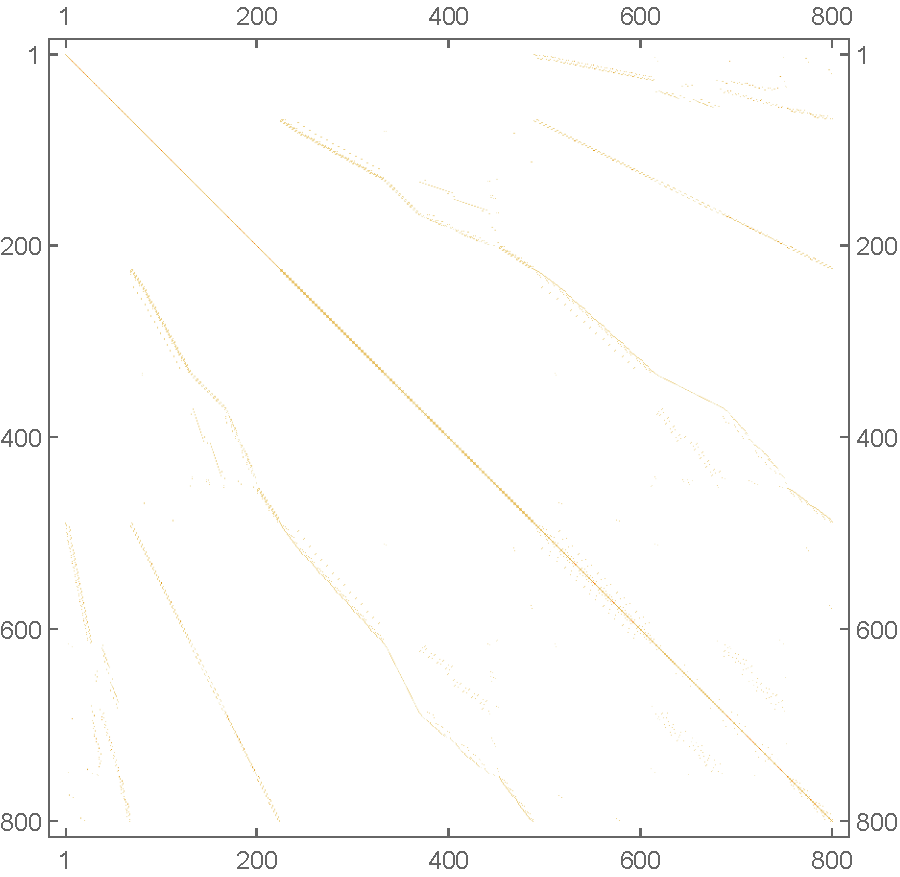
\includegraphics[width=\linewidth]{img/matrixPlotStrips.pdf}
	\caption{Портрет матрицы для рис.~(\ref{fig:matrixPlotStripsMesh})}\label{fig:matrixPlotStrips.pdf}
	\endminipage\hfill
	\minipage{0.4\textwidth}
	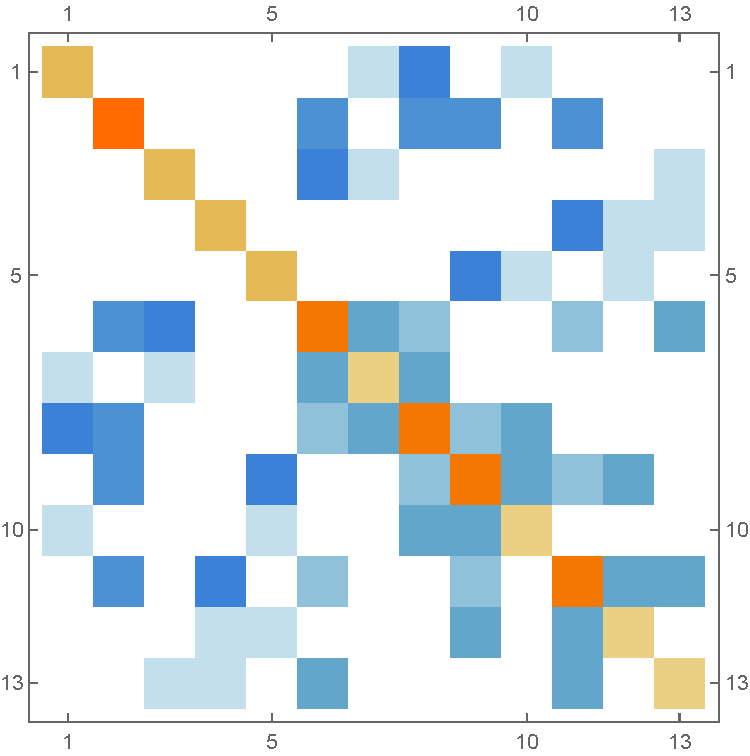
\includegraphics[width=\linewidth]{img/matrixPlotCircle.pdf}
	\caption{Портрет матрицы для рис.~(\ref{fig:matrixPlotCircleMesh})}\label{fig:matrixPlotCircle}
	\endminipage
\end{figure}

\begin{figure}[!hb]
	\minipage{0.4\textwidth}
	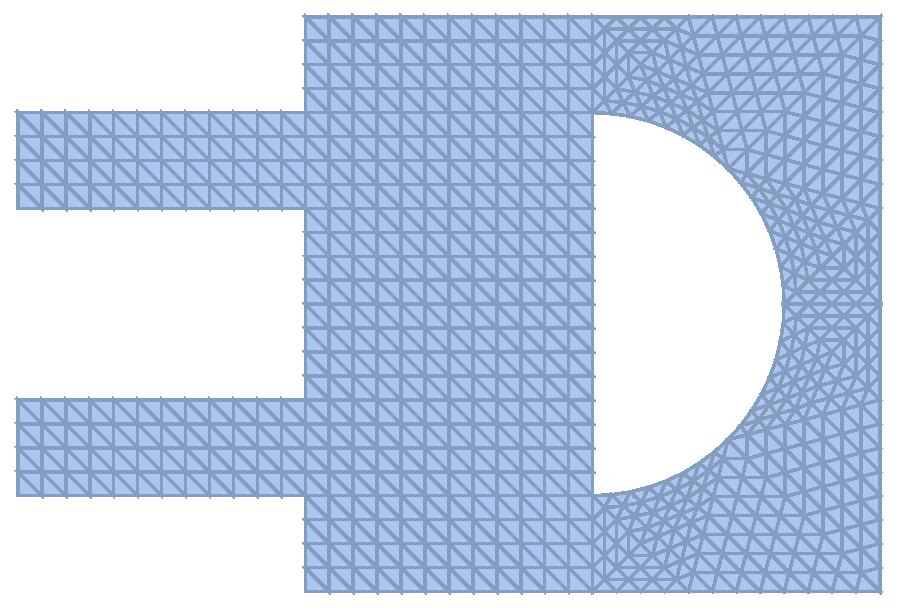
\includegraphics[width=\linewidth]{img/matrixPlotStripsMesh.pdf}
	\caption{Сетка с $n = 800$ для сложной области}\label{fig:matrixPlotStripsMesh}
	\endminipage\hfill
	\minipage{0.4\textwidth}
	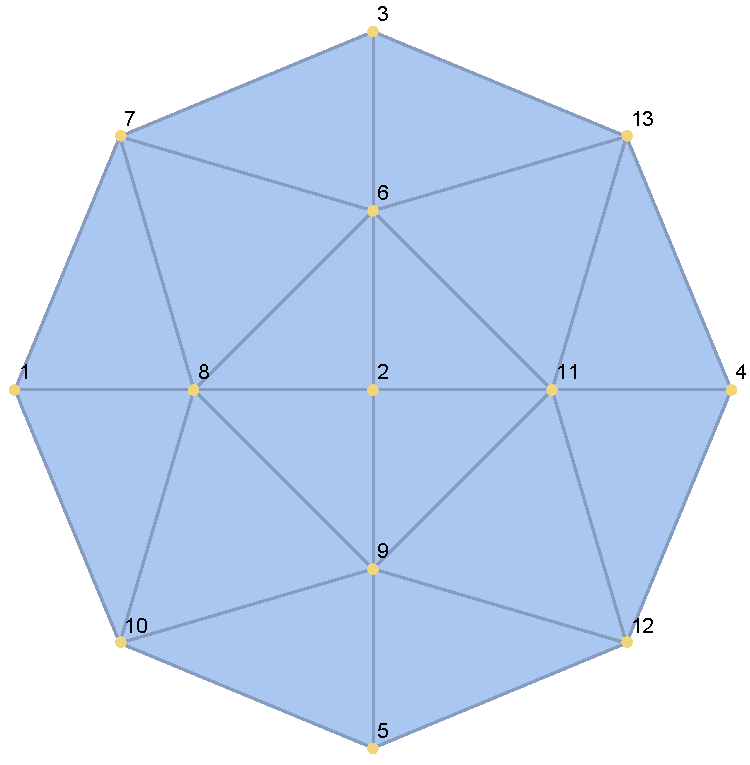
\includegraphics[width=\linewidth]{img/typicalMesh.pdf}
	\caption{Простая триангуляция круга}\label{fig:matrixPlotCircleMesh}
	\endminipage
\end{figure}

Можно показать, что для многих входных в~\ref{stationary} параметров матрица системы $\vect{A}$ будет положительно определена. Поэтому для решения СЛАУ разумно использовать \textbf{метод сопряжённых градиентов} (например, с $\vect{L} \, \vect{D} \, \vect{L}^T$--предобуславливанием).

Подробнее о реализации можно прочесть в~\cite{saad}.







    \newgeometry{left=2cm,right=1cm,top=1cm,bottom=1cm,includefoot,heightrounded}

\section{Задача, зависящая от времени}
\label{timeDependent}

Пусть дано \textbf{гиперболическое} уравнение
\begin{equation}
\label{hyperbolicEqn}
	\chi \, \ddot{u} + \sigma \, \dot{u} - \nabla \cdot (a \, \nabla u) = f, \quad \vect{x} \in \Omega, \quad t \in \left[ t_0, \, t_l \right],
\end{equation}
с краевыми условиями~(\ref{BCs}) и начальными условиями
\begin{subequations}
\label{ICs}
	\begin{align}
		u(\vect{x}, t_0) &= u_0(\vect{x}), \\
		\dot{u}(\vect{x}, t_0) &= v_0(\vect{x}).
	\end{align}
\end{subequations}

Отличия от~(\ref{eqn}~--~\ref{BCs}): здесь через «\,$\dot{}$\,» обозначена производная по времени $t$, входные параметры $\chi = \chi(\vect{x})$, $\sigma = \sigma(\vect{x})$ и $a = a(\vect{x})$ есть функции пространства, а $\kappa = \kappa(\vect{x}, \, t)$, $g_D = g_D(\vect{x}, \, t)$ и $g_N = g_N(\vect{x}, \, t)$ --- функции пространства и времени.\\
$u_0$ есть начальное положение, $v_0$ --- начальная скорость.

Через $\left[ t_0, \, t_l \right] \subset \left[ 0, \infty \right) $ обозначен временной сегмент, в котором нужно найти решение $u = u(\textbf{x}, \, t)$, удовлетворяющее~(\ref{hyperbolicEqn}~--~\ref{BCs}~--~\ref{ICs}).

Положив в~(\ref{hyperbolicEqn}) параметр $\chi \equiv 0$, получим задачу \textbf{параболического} типа. Поэтому все схемы решения, выведенные ниже, справедливы для задач и гиперболического, и параболического типа (с известными упрощениями).

\subsection{Вариационная постановка}

Подобно~(\ref{V}), определим пространство
\begin{equation}
\label{Vt}
	\mathbb{V}_t \coloneqq \{ v = v(\vect{x}, \, t): \normL{v(\cdot, t)} + \normL{\nabla v(\cdot, \, t)} < \infty \}.
\end{equation}

Аналогично тому, как мы поступили в разделе~\ref{Galerkin}, домножим уравнение~(\ref{hyperbolicEqn}) на тестовую функцию $v \in \mathbb{V}_t$, воспользуемся формулой Грина интегрирования по частям и краевыми условиями~(\ref{BCs}):
\begin{equation}
\label{hyperbolicVarForm}
	\overbrace{
		\int_{\Omega} \chi \, \ddot{u} \, v \diff{\vect{x}} +
		\int_{\Omega} \sigma \, \dot{u} \, v \diff{\vect{x}} +
		\int_{\Omega} a \, \nabla u \cdot \nabla v \diff{\vect{x}}  + 
		\int_{\partial \Omega} \kappa \, u \, v \diff{s}
	}^{\mathbcal{a}_t(u, v) \coloneqq}
	=
	\underbrace{
		\int_{\Omega} f \, v \diff{\vect{x}}  +
		\int_{\partial \Omega} ( \kappa \, g_D + g_N ) \, v \diff{s}.
	}_{\eqqcolon \mathbcal{l}_t(v)}
\end{equation}
Тогда слабая формулировка задачи~\ref{timeDependent}, аналогичная~(\ref{weakForm}), будет звучать так:
\begin{empheq}[box=\fbox]{align}
	\label{hyperbolicWeakForm}
	\begin{split}
		&\text{Найти пробную функцию } u \in \mathbb{V}_t, \text{ такую что равенство} \\
		&\mathbcal{a}_t(u, v) = \mathbcal{l}_t(v) \\
		&\text{справедливо для всех тестовых функций } v \in \mathbb{V}_t.
	\end{split}
\end{empheq}

Будем искать приближение $u_h$ в следующем виде:
\begin{equation}
\label{uht}
	u_h(\textbf{x}, \, t) = \sum_{1}^{n} \xi_i(t) \, \phi_i(x),
\end{equation}
т.\,е. предположим, что в каждый фиксированный момент времени $t$ наше решение есть житель конечномерного кусочно--линейного непрерывного на $\Omega_h$ подпространства $\mathbb{V}_h$, определённого в разделе~\ref{chooseVh}.

Подставляя представление~(\ref{uht}) в~\ref{hyperbolicWeakForm} и (учитывая конечномерность пространства $\mathbb{V}_h$) заменяя тестовую функцию на базисную, получим:
\begin{align*}
	&\sum_{i=1}^n \Bigg( 
		\ddot{\xi}_i(t) \int_{\Omega} \chi \, \phi_i \, \phi_j \diff{\vect{x}} +
		\dot{\xi}_i(t) \int_{\Omega} \sigma \, \phi_i \, \phi_j \diff{\vect{x}} +
		\xi_i(t) \bigg(
			\int_{\Omega} a \, \nabla \phi_i \, \nabla \phi_j \diff{\vect{x}} +
			\int_{\partial \Omega} \kappa \, \phi_i \, \phi_j \diff{s}
		\bigg)
	\Bigg)
	= \\
	&\int_{\Omega} f \, \phi_j \diff{\vect{x}}  +
	\int_{\partial \Omega} ( \kappa \, g_D + g_N ) \, \phi_j \diff{s}
	\qquad \text{ для всех } \phi_j, \quad j = 1, \, 2, \, \dots, \, n, 
\end{align*}
что есть ничто иное, как система линейных дифференциальных уравнений (СЛДУ)
\begin{equation}
\label{SLDE}
	\vect{M}^\chi \, \ddot{\vect{\xi}} +
	\vect{M}^\sigma \, \dot{\vect{\xi}} + 
	\big( \vect{S} + \vect{R}(t) \big) \, \vect{\xi}
	=
	\vect{f}(t) + \vect{r}(t),
\end{equation}
где $\vect{\xi}(t) \coloneqq \big( \xi_1(t), \, \xi_2(t), \, \dots, \, \xi_n(t) \big)^T$ --- вектор неизвестных функций--весов, $\vect{M}^\chi$ и $\vect{M}^\sigma$ суть привычные матрицы масс (см.~(\ref{how2compute})) с входящими в интегранд $\chi$ и $\sigma$ соответственно, $\vect{S}$ --- матрица жёсткости, $\vect{R}$ --- матрица Робина, $\vect{f}$ --- вектор нагрузки и $\vect{r}$ --- вектор Робина.

\subsection{Решение СЛДУ методом Крэнка---Николсона (\texttt{CN3}) и неявной трёхслойной схемой (\texttt{BDF3})}

Выберем $l-1$ точку $t_1, \, t_2, \, \dots, \, t_{l-1}$ так, что $t_0 < t_1 < \dots < t_{l-1} < t_l$. Точки--элементы списка $T_l \coloneqq \langle \, t_0, \, t_1, \, \dots, \, t_l \, \rangle$ назовём \textbf{временными слоями} и будем искать решение в них. 

Классический способ решения СЛДУ --- метод конечных разностей (МКР). Предполагая константный временной шаг $\Delta t_m \coloneqq t_m - t_{m-1}$, аппроксимируем дифференциальные операторы 

\begin{subequations}
\label{finiteDiffConstOps}
	\begin{align}
		\ddot{\vect{\xi}}(t_m) &= \frac{\vect{\xi}(t_m) - 2 \, \vect{\xi}(t_{m-1}) + \vect{\xi}(t_{m-2})}{\Delta t^2} + O(\Delta t^3), 
		\\
		\dot{\vect{\xi}}(t_m) &= \frac{\vect{\xi}(t_m) - \vect{\xi}(t_{m-2})}{2 \, \Delta t} + O(\Delta t^3)
	\end{align}
\end{subequations}
в системе~(\ref{SLDE}) на $m$--м временном слое:
\begin{subequations}
\label{finiteDiffConstConst}
	\begin{align}
		&
		\vect{M}^\chi \, \frac{\vect{\xi}^m - 2 \, \vect{\xi}^{m-1} + \vect{\xi}^{m-2}}{\Delta t^2} +
		\vect{M}^\sigma \, \frac{\vect{\xi}^m - \vect{\xi}^{m-2}}{2 \, \Delta t} + \nonumber \\ 
		&
		\vect{S} \, \frac{\vect{\xi}^m + \vect{\xi}^{m-2}}{2} +
		\frac{1}{2} \, \Big( \vect{R}(t_m) \, \vect{\xi}^m + \vect{R}(t_{m-2}) \, \vect{\xi}^{m-2} \Big)
		= 
		\frac{1}{2} \, \Big( \vect{f}(t_m) + \vect{f}(t_{m-2}) + \vect{r}(t_m) + \vect{r}(t_{m-2}) \Big), \label{CN3const} \\
		&
		\vect{M}^\chi \, \frac{\vect{\xi}^m - 2 \, \vect{\xi}^{m-1} + \vect{\xi}^{m-2}}{\Delta t^2} +
		\vect{M}^\sigma \, \frac{\vect{\xi}^m - \vect{\xi}^{m-2}}{2 \, \Delta t} + 
		\Big( \vect{S} + \vect{R}(t_m) \Big) \, \vect{\xi}^m
		= 
		\vect{f}(t_m) + \vect{r}(t_m). \label{BDF3const}
	\end{align}
\end{subequations}
Разностная схема~(\ref{CN3const}) называется \textbf{трёхслойной схемой Крэнка---Николсона} (\textit{Crank---Nicolson scheme}, \texttt{CN3}), а разностная схема~(\ref{BDF3const}) --- \textbf{трёхслойной неявной схемой} (\textit{Backward difference formula}, \texttt{BDF3}).  

Снимем предположение о константности временного шага $\Delta t_m$. Вывести аналог трёхслойных разностных операторов~(\ref{finiteDiffConstOps}) для первой и второй производной проще всего в терминах так называемого \textit{временного базиса}.

Ясно, что для полиномов второго порядка ошибка аппроксимации $O(\Delta t^3)$ в~(\ref{finiteDiffConstOps}) равна нулю\footnote{
	Четвёртый член ряда Тейлора включает в себя третью производную, которая равна нулю у функций вида $c_1 \, t^2 + c_2 \, t + c_3$; производные высших порядков также дадут ноль. Поэтому дифференциальный и разностный операторы в~(\ref{finiteDiffConstOps}) будут совпадать.
}. Предположим, что на отрезке $\left[ t_{m-2}, \, t_{m} \right]$ вектор весов есть некоторая квадратичная функция, $\vect{\xi}|_{\left[ t_{m-2}, \, t_{m} \right]} \in \spn \, \{ \, t^2, \, t, \, 1 \, \} = \spn \, \{ \, \eta^{m-2}(t), \, \eta^{m-1}(t), \, \eta^{m}(t) \, \}$. \\ 
Здесь $\eta^{m-2}(t)$, $\eta^{m-1}(t)$ и $\eta^{m}(t)$ есть квадратичные функции вершинного временного базиса, такие что $\eta^{m-j}(t_{m-k}) = \delta_{j \, k}$ (см. рис.~\ref{fig:timeBasis}). Их аналитический вид легко получить аналогично~(\ref{basisCoef}).

Тогда  $\vect{\xi}(t)$ можно представить в виде
\begin{equation*}
	\vect{\xi}(t) = \eta^{m-2}(t) \, \vect{\xi}(t_{m-2}) + \eta^{m-1}(t) \, \vect{\xi}(t_{m-1}) + \eta^{m}(t) \, \vect{\xi}(t_{m}), \quad t \in \left[ t_{m-2}, \, t_{m} \right]
\end{equation*} 
и разностные схемы~(\ref{finiteDiffConstConst}) будут иметь вид
\begin{subequations}
	\label{finiteDiffConst}
	\begin{align}
		&
		\vect{M}^\chi \, \sum_{k=0}^2 \ddot{\eta}^{m-k}(t_m) \, \vect{\xi}^{m-k} +
		\vect{M}^\sigma \, \sum_{k=0}^2 \dot{\eta}^{m-k}(t_m) \, \vect{\xi}^{m-k} +
		\vect{S} \, \frac{\vect{\xi}^m + \vect{\xi}^{m-2}}{2} + \nonumber \\
		&
		\frac{1}{2} \, \Big( \vect{R}(t_m) \, \vect{\xi}^m + \vect{R}(t_{m-2}) \, \vect{\xi}^{m-2} \Big)
		= 
		\frac{1}{2} \, \Big( \vect{f}(t_m) + \vect{f}(t_{m-2}) + \vect{r}(t_m) + \vect{r}(t_{m-2}) \Big), \label{CN3} \\
		&
		\vect{M}^\chi \, \sum_{k=0}^2 \ddot{\eta}^{m-k}(t_m) \, \vect{\xi}^{m-k} +
		\vect{M}^\sigma \, \sum_{k=0}^2 \dot{\eta}^{m-k}(t_m) \, \vect{\xi}^{m-k} +
		\Big( \vect{S} + \vect{R}(t_m) \Big) \, \vect{\xi}^m 
		= 
		\vect{f}(t_m) + \vect{r}(t_m). \label{BDF3}
	\end{align}
\end{subequations}

Очевидно, решение по обеим схемам эквивалентно решению последовательности СЛАУ вида
\begin{equation*}
	\vect{A}^m \, \vect{\xi}^m = \vect{b}^m, \quad m = 2, \, 3, \, \dots, \, l.
\end{equation*} 
Для~(\ref{CN3}) имеем
\begin{subequations}
	\label{CN3_Ab}
	\begin{align}
		\vect{A}^m &=
		\ddot{\eta}^{m}(t_m) \, \vect{M}^\chi +
		\dot{\eta}^{m}(t_m) \, \vect{M}^\sigma +
		\frac{1}{2} \, \Big(
			\vect{S} +
			\vect{R}(t_m) 
		\Big), \label{CN3_A} 
		\\
		\vect{b}^m &=
		\frac{1}{2} \, \Big( 
				\vect{f}(t_m) + \vect{f}(t_{m-2}) + 
				\vect{r}(t_m) + \vect{r}(t_{m-2}) -
				\big( \vect{S} + \vect{R}(t_{m-2}) \big) \, \vect{\xi}^{m-2}
			\Big) \nonumber \\
		&-
		\ddot{\eta}^{m-1}(t_m) \, \vect{M}^\chi \, \vect{\xi}^{m-1} -
		\ddot{\eta}^{m-2}(t_m) \, \vect{M}^\chi \, \vect{\xi}^{m-2} \nonumber \\
		&-
		\dot{\eta}^{m-1}(t_m) \, \vect{M}^\sigma \, \vect{\xi}^{m-1} -
		\dot{\eta}^{m-2}(t_m) \, \vect{M}^\sigma \, \vect{\xi}^{m-2}, \label{CN3_b} 
	\end{align}
\end{subequations}
a для~(\ref{BDF3}) ---
\begin{subequations}
	\label{BDF3_Ab}
	\begin{align}
		\vect{A}^m &=
		\ddot{\eta}^{m}(t_m) \, \vect{M}^\chi +
		\dot{\eta}^{m}(t_m) \, \vect{M}^\sigma +
		\vect{S} +
		\vect{R}(t_m), \label{BDF3_A} 
		\\
		\vect{b}^m &=
		\vect{f}(t_m) + 
		\vect{r}(t_m) \nonumber \\
		&-
		\ddot{\eta}^{m-1}(t_m) \, \vect{M}^\chi \, \vect{\xi}^{m-1} - 
		\ddot{\eta}^{m-2}(t_m) \, \vect{M}^\chi \, \vect{\xi}^{m-2} \nonumber \\
		&-
		\dot{\eta}^{m-1}(t_m) \, \vect{M}^\sigma \, \vect{\xi}^{m-1} -
		\dot{\eta}^{m-2}(t_m) \, \vect{M}^\sigma \, \vect{\xi}^{m-2}. \label{BDF3_b} 
	\end{align}
\end{subequations}
Аналитический вид производных временного базиса доступен в~\ref{timeBasisDer}.

Для начала работы схемы необходимы векторы $\vect{\xi}^0$ и $\vect{\xi}^1$. Воспользуемся начальными условиями~(\ref{ICs}) и положим
\begin{subequations}
\label{xi01}
	\begin{align}
		\xi^0_i &= u(\vect{x}_i, \, t_0) = u_0(\vect{x}_i), \\
		\xi^1_i &= u(\vect{x}_i, \, t_1) \simeq 
		u(\vect{x}_i, \, t_0) + \dot{u}(\vect{x}_i, \, t_0) \, \Delta t_1 \nonumber \\
		&= \vect{x}_i + v_0(\vect{x}_i) \, \Delta t_1,
		\quad \vect{x}_1, \, \vect{x}_2, \, \dots, \, \vect{x}_n \text{ --- узлы сетки } \Omega_h. \label{xi1}
	\end{align}
\end{subequations}
Погрешность аппроксимации в~(\ref{xi1}) есть $O(\Delta t_1^2)$, что на порядок ниже, чем погрешность аппроксимации в~(\ref{finiteDiffConstOps}). Поэтому при анализе порядка сходимости на модельных задачах (задачах с известным аналитическим решением) в разделе~\ref{hyperbolicTests} мы положим
\begin{equation*}
	\xi^1_i = u(\vect{x}_i, \, t_1).
\end{equation*}
Процесс генерации портрета матрицы, сборки СЛАУ, --- учёт вноса вкладов от локальных матриц и векторов, --- и процесс решения аналогичны тому, это описывалось в секции~\ref{steadyState}, поэтому мы не будем обсуждать это здесь.

\subsubsection{Формулы для производных временного базиса}
\label{timeBasisDer}

$$
	\begin{matrix*}[l]
		\dot{\eta}^{m-2}(t_m) =
			\frac{t_m - t_{m-1}}{\left(t_{m-2}-t_{m-1}\right) \left(t_{m-2}-t_m\right)} \quad
		&
		\ddot{\eta}^{m-2}(t_m) =
			\frac{2}{\left(t_{m-2}-t_{m-1}\right) \left(t_{m-2}-t_m\right)} 
		\\
		\dot{\eta}^{m-1}(t_m) =
			\frac{t_{m-2}-t_m}{\left(t_{m-2}-t_{m-1}\right) \left(t_{m-1}-t_m\right)}
		&
		\ddot{\eta}^{m-1}(t_m) =
			\frac{2}{\left(t_{m-2}-t_{m-1}\right) \left(t_m-t_{m-1}\right)} 
		\\
		\dot{\eta}^{m}(t_m) =
			\frac{t_{m-2}+t_{m-1}-2 t_m}{\left(t_{m-2}-t_m\right) \left(t_m-t_{m-1}\right)}
		&
		\ddot{\eta}^{m}(t_m) =
			\frac{2}{\left(t_{m-2}-t_m\right) \left(t_{m-1}-t_m\right)}
	\end{matrix*}
$$

\begin{figure}[!h]
	\centering
	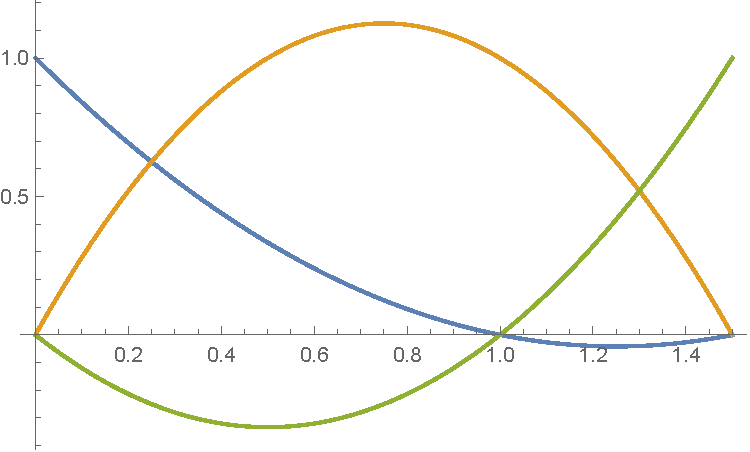
\includegraphics[width=0.8\linewidth]{img/timeBasis.pdf}
	\caption{Функции временного базиса $\eta^{m-2}(t)$, $\eta^{m-1}(t)$ и $\eta^{m}(t)$, $t_{m-2} = 0$, $t_{m-1} = 1$ и $t_{m-1} = 1.5$}
	\label{fig:timeBasis}
\end{figure}

\subsection{Тестирование на модельных задачах}
\label{hyperbolicTests}

\subsubsection{Расчётная область}

Следующие в разделе~\ref{hyperbolicTests} модельные задачи будут решены на триангуляции $\Omega_h$, построенной для квадрата $\Omega$ с вершинами $(0, \, 0)$, $(1, \, 0)$, $(1, \, 1)$ и $(0, \, 1)$ и с краевыми условиями всех типов (см. рис.~\ref{fig:modelSquare}).

\begin{figure}[!h]
	\centering
	\resizebox{0.5\textwidth}{!}{\input{img/modelSquare.pdf_tex}}
	\caption{Расчётная область $\Omega_h$}
	\label{fig:modelSquare}
\end{figure}

\subsubsection{Априорная оценка ошибки}

Известно, что численное решение~(см.~\cite[с.~124]{umea}) удовлетворяет
\begin{align}
\label{estimate}
	\normL{u(\cdot, \, t_m) - u_h(\cdot, \, t_m)} & \le
	C \, h^2 \, \Big( 
		\normL{u''_0} + \int_{t_0}^{t_l} \normL{\dot{u}''(\cdot, \, s)} \diff{s}
	\Big) \nonumber \\
	& + C \, k \, \int_{t_0}^{t_l} \normL{\ddot{u}''(\cdot, \, s)} \diff{s},
\end{align}
где $h \coloneqq$ максимальная длина ребра триангуляции $\Omega_h$. \\
Отсюда видно, что имеет место \textbf{2-й порядок сходимости по пространству и 1-й --- по времени}.

Далее мы попробуем на модельных задачах апостериорно установить порядок сходимости по времени и пространству в смысле 2--нормы.

\subsubsection{«Простая» задача}
\label{simple}

Рассмотрим сначала задачу
\begin{equation}
	2 \, \ddot{u} + \dot{u} -  \nabla^2 \, u = 2 \, (2 + t), \quad \vect{x} \in \Omega, \quad t \in \left[ 0, \, 1 \right],
\end{equation}
c краевыми условиями
\begin{align*}
	(-1, \, 0) \cdot \nabla u + u &= t^2 + x - 2 \, y - 1, \quad & \vect{x} \in \Gamma_R, & \qquad \qquad \qquad \qquad \\
	(1, \, 0) \cdot \nabla u &= 1, & \vect{x} \in \Gamma_N, & \\
	u &= t^2 + x - 2 \, y, & \vect{x} \in \Gamma_{D_1} \cup \Gamma_{D_1}, &
\end{align*}
и начальными условиями
\begin{align*}
	u(\vect{x}, 0) &= x - 2 \, y, \\
	\dot{u}(\vect{x}, 0) &= 0.
\end{align*}
Она имеет аналитическое решение $u(\vect{x}, t) = t^2 + x - 2 \, y$.

\paragraph{Решение по схеме \texttt{CN3}}

\renewcommand{\arraystretch}{2}
\begin{table}[H]
	\caption{Решение «простой»~\ref{simple} задачи по схеме \texttt{CN3}, дробление по времени}
	\label{tab:CN3plain}
	\begin{center}\begin{tabular}{|c|c|c|c|c|c|c|}
		\hline
		$h$ & $n$ & $\Delta t$ & $l$ & $\Delta_h$ & $\delta_h$ & $\frac{\delta_{2 \, h}}{\delta_h}$ \\
		\hline
		$\frac{\sqrt{2}}{6}$ & 49 & $\frac{1}{2}$ & 3 & $3.62 \times 10^{-1}$ & $5.76 \times 10^{-2}$ & \\
		\hline
		$\frac{\sqrt{2}}{6}$ & 49 & $\frac{1}{8}$ & 9 & $1.8 \times 10^{-1}$ & $2.86 \times 10^{-2}$ & 2.01 \\
		\hline
		$\frac{\sqrt{2}}{6}$ & 49 & $\frac{1}{32}$ & 33 & $4.87 \times 10^{-2}$ & $7.79 \times 10^{-3}$ & 3.67 \\
		\hline
		$\frac{\sqrt{2}}{6}$ & 49 & $\frac{1}{128}$ & 129 & $1.24 \times 10^{-2}$ & $1.99 \times 10^{-3}$ & 3.92 \\
		\hline
		$\frac{\sqrt{2}}{6}$ & 49 & $\frac{1}{512}$ & 513 & $3.11 \times 10^{-3}$ & $4.99 \times 10^{-4}$ & 3.98 \\
		\hline
	\end{tabular}\end{center}
\end{table}
\begin{table}[H]
	\caption{Решение «простой» задачи~\ref{simple} по схеме \texttt{CN3}, дробление по времени и пространству}
	\label{tab:CN3plainFull}
	\begin{center}\begin{tabular}{|c|c|c|c|c|c|c|}
		\hline
		$h$ & $n$ & $\Delta t$ & $l$ & $\Delta_h$ & $\delta_h$ & $\frac{\delta_{2 \, h}}{\delta_h}$ \\
		\hline
		$\frac{\sqrt{2}}{3}$ & 16 & $\frac{1}{2}$ & 3 & $2. \times 10^{-1}$ & $5.16 \times 10^{-2}$ & \\
		\hline
		$\frac{\sqrt{2}}{6}$ & 49 & $\frac{1}{8}$ & 9 & $1.8 \times 10^{-1}$ & $2.86 \times 10^{-2}$ & 1.8 \\
		\hline
		$\frac{\sqrt{2}}{12}$ & 169 & $\frac{1}{32}$ & 33 & $9.33 \times 10^{-2}$ & $8.45 \times 10^{-3}$ & 3.38 \\
		\hline
		$\frac{\sqrt{2}}{24}$ & 625 & $\frac{1}{128}$ & 129 & $4.65 \times 10^{-2}$ & $2.26 \times 10^{-3}$ & 3.74 \\
		\hline
		$\frac{\sqrt{2}}{48}$ & 2401 & $\frac{1}{512}$ & 513 & $2.31 \times 10^{-2}$ & $5.84 \times 10^{-4}$ & 3.88 \\
		\hline
	\end{tabular}\end{center}
\end{table}
Поясним нотации в таблицах~\ref{tab:CN3plain}~--~\ref{tab:CN3plainFull}:
\begin{itemize}
	\item $h$ --- максимальная длина ребра сетки $\Omega_h$,
	\item $n$ --- количество узлов триангуляции (размерность СЛАУ, решаемой на каждом временном слое $t_m$),
	\item $\Delta t$ --- размер шага по времени,
	\item $l$ --- количество временных слоёв,
	\item $\Delta_h \coloneqq \max_{\, 0 \le m \le l \,} \norm{\vect{u}^m - \vect{\xi}^m}_2$ --- максимальная 2-норма ошибки, \\ 
	      $\vect{u}^m \coloneqq ( u^m(\vect{x}_1), \, u^m(\vect{x}_2), \, \dots, \, u^m(\vect{x}_n) )$ --- вектор значений точного решения $u$ на $m$--м временном слое,
	\item $\delta_h \coloneqq \max_{\, 0 \le m \le l \,} \frac{\norm{\vect{u}^m - \vect{\xi}^m}_2}{\norm{\vect{u}^m}_2}$ --- максимальная относительная погрешность и 
	\item $\frac{\delta_{2 \, h}}{\delta_h}$ --- отношение предыдущей относительной погрешности к текущей.
\end{itemize}

\paragraph{Решение по схеме \texttt{BDF3}}

Решение по схеме \texttt{BDF3} сразу же при $n = 49$ и $m = 3$ (см. первую строку таблиц~\ref{tab:CN3plain}~--~\ref{tab:CN3plainFull}) даёт ошибку $\Delta_h = 3.21 \times 10^{-15}$ и относительную ошибку $\delta_h = 5.12 \times 10^{-16}$, которые сохраняются незначительными с дроблением временного шага.

\begin{figure}[!h]
	\minipage{0.45\textwidth}
	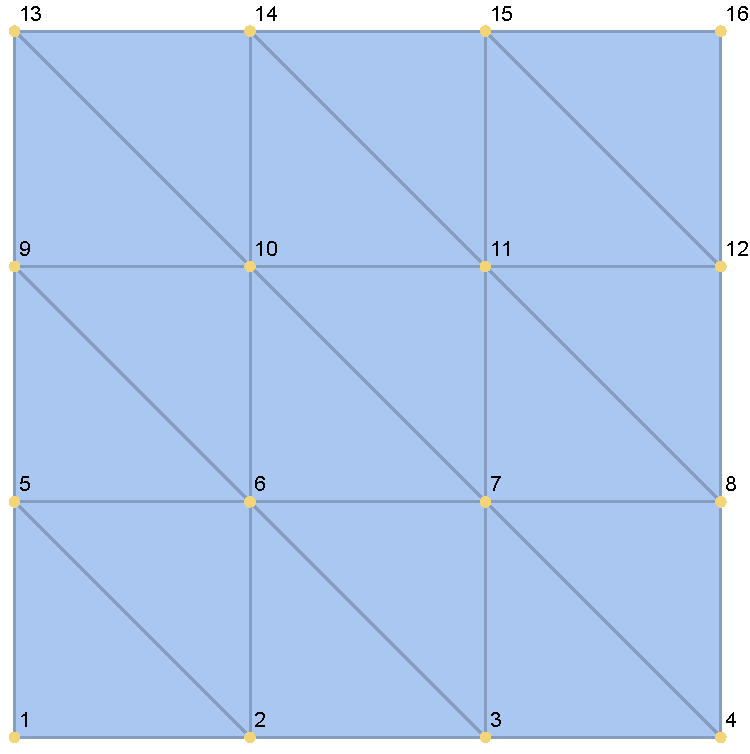
\includegraphics[width=\linewidth]{img/n16mesh.pdf}
	\caption{Сетка $\Omega_h$ из 2--й строки таблицы~\ref{tab:CN3plainFull}, $h = \frac{\sqrt{2}}{3}$ и \dots}\label{fig:n16mesh}
	\endminipage\hfill
	\minipage{0.45\textwidth}
	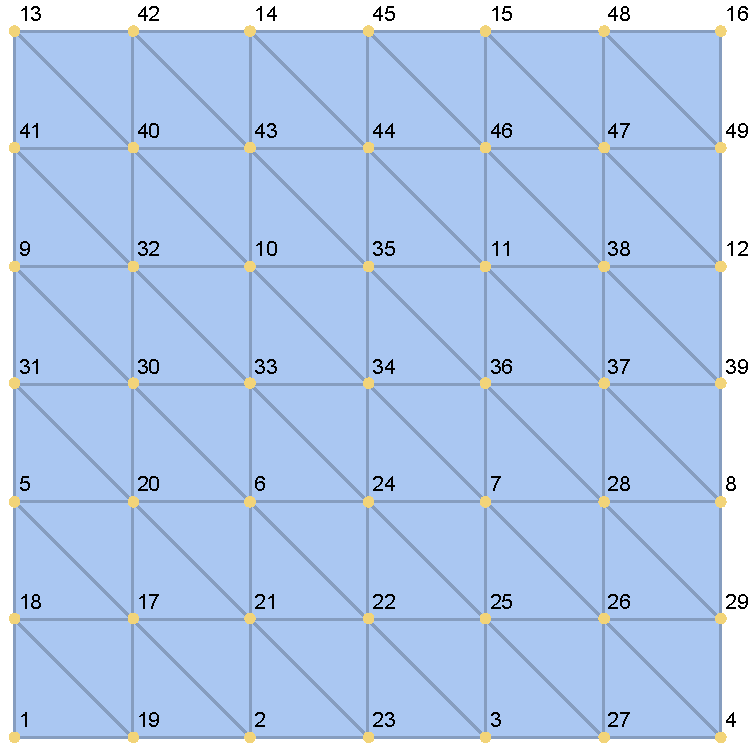
\includegraphics[width=\linewidth]{img/n49mesh.pdf}
	\caption{\dots измельчённая сетка из 3--й строки, $h = \frac{\sqrt{2}}{6}$}\label{fig:n49mesh}
	\endminipage
\end{figure}

\subsubsection{«Косинус--волна»}
\label{cosWave}

Рассмотрим теперь задачу
\begin{align*}
	& \ddot{u} + .1 \, \dot{u} -  \nabla \cdot (x \, y \, \nabla u) = \\
	& 5 \, (x + y - .1) \, \sin \big( 5 \, (t + x + y) \big) + 25 (2 \, x \, y - 1) \, \cos \big( 5 \, (t + x + y) \big), \\
	& \vect{x} \in \Omega, \quad t \in \left[ 0, \, 1 \right],
\end{align*}
c краевыми условиями
\begin{align*}
	(-1, \, 0) \cdot \nabla u + u &= 5 \, x \, y \, \sin \big( 5 \, (t + x + y) \big) + \cos \big( 5 \, (t + x + y) \big), & \vect{x} \in \Gamma_R, & \qquad \qquad \\
	(1, \, 0) \cdot \nabla u &= -5 \, x \, y \, \sin \big( 5 \, (t + x + y) \big), & \vect{x} \in \Gamma_N, & \\
	u &= \cos \big( 5 \, (t + x + y) \big), & \vect{x} \in \Gamma_{D_1} \cup \Gamma_{D_1}, &
\end{align*}
и начальными условиями
\begin{align*}
	u(\vect{x}, 0) &= \cos \big( 5 \, (x + y) \big), \\
	\dot{u}(\vect{x}, 0) &= -5 \sin \big( 5 \, (x + y) \big).
\end{align*}
Она имеет аналитическое решение $u(\vect{x}, t) = \cos \big( 5 \, (t + x + y) \big)$.

\paragraph{Решение по схеме \texttt{CN3}}

\begin{table}[H]
\caption{Решение задачи~\ref{cosWave} по схеме \texttt{CN3}, дробление по времени и пространству}
\label{tab:CN3cosWaveFull}
	\begin{center}\begin{tabular}{|c|c|c|c|c|c|c|}
		\hline
		$h$ & $n$ & $\Delta t$ & $l$ & $\Delta_h$ & $\delta_h$ & $\frac{\delta_{2 \, h}}{\delta_h}$ \\
		\hline
		$\frac{\sqrt{2}}{2}$ & 9 & $\frac{1}{2}$ & 3 & $4.15$ & $1.86$ & \\
		\hline
		$\frac{\sqrt{2}}{4}$ & 25 & $\frac{1}{8}$ & 9 & $7.4 \times 10^{-1}$ & $2.09 \times 10^{-1}$ & 8.87 \\
		\hline
		$\frac{\sqrt{2}}{8}$ & 81 & $\frac{1}{32}$ & 33 & $4.27 \times 10^{-1}$ & $6.7 \times 10^{-2}$ & 3.13 \\
		\hline
		$\frac{\sqrt{2}}{16}$ & 289 & $\frac{1}{128}$ & 129 & $2.6 \times 10^{-1}$ & $2.15 \times 10^{-2}$ & 3.11 \\
		\hline
		$\frac{\sqrt{2}}{32}$ & 1089 & $\frac{1}{512}$ & 513 & $1.36 \times 10^{-1}$ & $5.78 \times 10^{-3}$ & 3.72 \\
		\hline
	\end{tabular}\end{center}
\end{table}

\paragraph{Решение по схеме \texttt{BDF3}}

\begin{table}[H]
\caption{Решение задачи~\ref{cosWave} по схеме \texttt{BDF3}, дробление по времени и пространству}
\label{tab:BDF3cosWaveFull}
	\begin{center}\begin{tabular}{|c|c|c|c|c|c|c|}
		\hline
		$h$ & $n$ & $\Delta t$ & $l$ & $\Delta_h$ & $\delta_h$ & $\frac{\delta_{2 \, h}}{\delta_h}$ \\
		\hline
		$\frac{\sqrt{2}}{2}$ & 9 & $\frac{1}{2}$ & 3 & $2.88$ & $1.29$ & \\
		\hline
		$\frac{\sqrt{2}}{4}$ & 25 & $\frac{1}{8}$ & 9 & $4.63$ & $1.31$ & 0.985 \\
		\hline
		$\frac{\sqrt{2}}{8}$ & 81 & $\frac{1}{32}$ & 33 & $2.57$ & $4.02 \times 10^{-1}$ & 3.25 \\
		\hline
		$\frac{\sqrt{2}}{16}$ & 289 & $\frac{1}{128}$ & 129 & $1.34$ & $1.11 \times 10^{-1}$ & 3.64 \\
		\hline
		$\frac{\sqrt{2}}{32}$ & 1089 & $\frac{1}{512}$ & 513 & $6.71 \times 10^{-1}$ & $2.86 \times 10^{-2}$ & 3.87 \\
		\hline
	\end{tabular}\end{center}
\end{table}

\begin{figure}[!hb]
	\minipage{0.45\textwidth}
	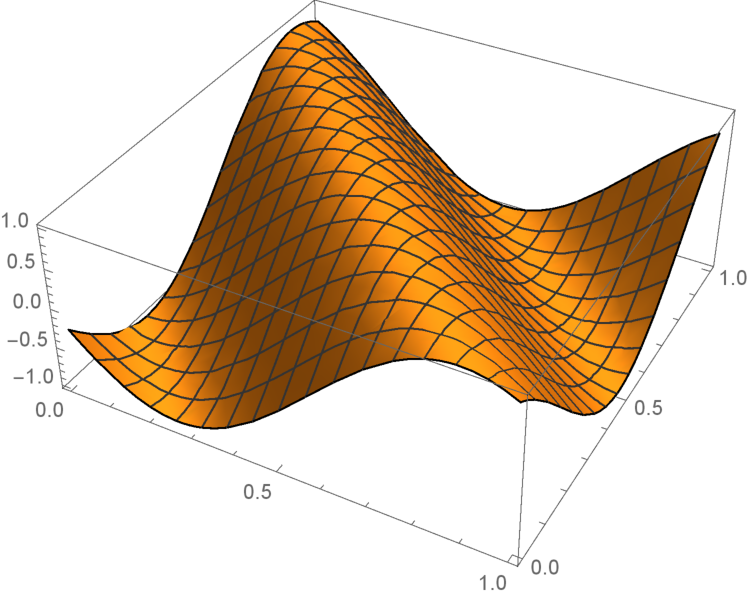
\includegraphics[width=\linewidth]{img/cosWaveAnalytic.pdf}
	\caption{Аналитическое решение $u(\vect{x}, \, .375) = \cos \big( 5 \, (.375 + x + y) \big)$ задачи~\ref{cosWave} и \dots}\label{fig:cosWaveAnalytic.pdf}
	\endminipage\hfill
	\minipage{0.45\textwidth}
	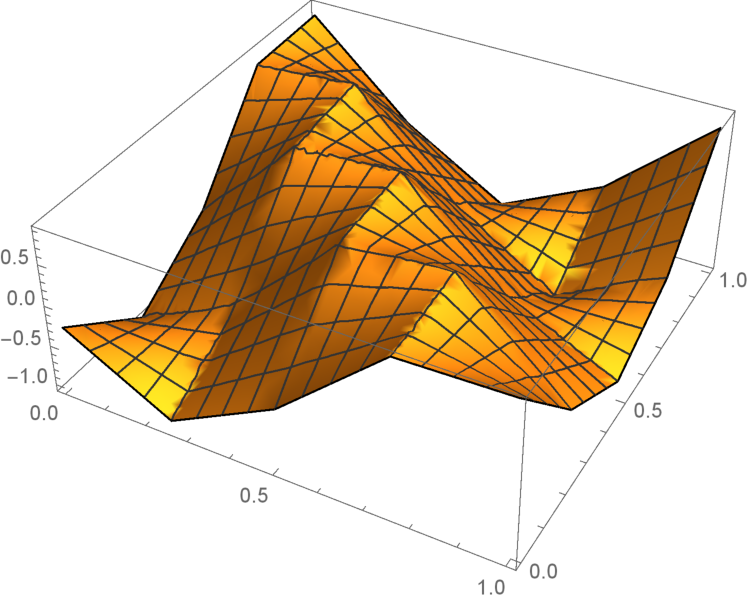
\includegraphics[width=\linewidth]{img/cosWaveNumeric.pdf}
	\caption{\dots численное решение $u_h$ на 4--м временном слое $t_4 = .375$, определённое на сетке с $n = 25$ узлами --- см. 3--ю строку таблицы~\ref{tab:CN3cosWaveFull}}\label{fig:cosWaveNumeric}
	\endminipage
\end{figure}

\subsubsection{Выводы}

Главное, на что следует обратить внимание в решениях модельных задач~\ref{simple} и~\ref{cosWave}:
\begin{itemize}
	\item Во всех таблицах (за исключением~\ref{tab:CN3plain}) видно, что мы дробим шаг по пространству $h$ в два раза, а шаг по времени $\Delta t$ --- в четыре. При этом ясно наблюдается сходимость отношения максимумов относительных погрешностей к четырём.\\
	Отсюда делаем вывод, что \textbf{численное решение $u_h$ в смысле 2-нормы сходится к аналитическому со вторым порядком по пространству и с первым --- по времени} (см. априорную оценку~(\ref{estimate})).\\
	Сходимость справедлива для обоих тестов.
	\item Очевидно, что решение задачи~\ref{simple} $u(\vect{x}, t) = t^2 + x - 2 \, y$ для любого $t$ есть житель подпространства $\mathbb{V}_h$, в котором мы ищем приближение к аналитическому решению. Стало быть нет необходимости в дроблении пространственной сетки (и, как следствие, в нагрузке на ресурсы компьютера) --- на скорость сходимости это не влияет, как видно из таблиц~\ref{tab:CN3plain} и~\ref{tab:CN3plainFull}.
	\item На «простом» тесте~\ref{simple} \texttt{CN3} сработала гораздо хуже \texttt{BDF3}, однако
	\item для уравнения с «косинус--волной»~\ref{cosWave} «усреднённые»\footnote{
			Говорят, что схемы типа Крэнка--Николсона отражают закон сохранения энергии, свойственный некоторым волновым уравнениям, не давая решению «расплываться» --- см.~\cite[с.~137]{umea}.
		} вклады от соседних временных слоёв в~(\ref{BDF3_Ab}) дали о себе знать: погрешность $\Delta_h = 1.36 \times 10^{-1}$ метода \texttt{CN3} в 5 раз меньше, чем погрешность $\Delta_h = 6.71 \times 10^{-1}$ метода \texttt{BDF3}. Более того, из таблицы~\ref{tab:BDF3cosWaveFull} видно, что только на самом мелком шаге по времени и пространству погрешность метода \texttt{BDF3} упала до второго знака;
	\item отсюда делаем вывод, что --- хотя оба метода обладают одним порядком сходимости --- скорость сходимости может очень сильно зависеть от конкретной задачи. 
\end{itemize}

\newpage
\subsection{Исходный текст программы}

Здесь мы приведём основной модуль --- пространство имён \texttt{FEMt}, содержащее решатели \texttt{CN3} и \texttt{BDF3} и вспомогательные функции для расчёта локальных матриц и векторов. Весь комплекс программ, как было отмечено в начале, доступен в репозитории:
\url{https://github.com/CATSPDEs} \\

\lstinputlisting[language=C++]{FEMt.cpp}

    \newpage
    \begin{thebibliography}{99}
\bibitem{PDEs} Walter A. Strauss\\
	\textit{Partial Differential Equations: an Introduction}\\
	Brown University\\
	John Wiley \& Sons, 2008
\bibitem{umea} Mats G. Larson, Fredrik Bengzon\\
    \textit{The Finite Element Method: Theory, Implementation, and Applications}\\
    Department of Mathematics, Umeå University\\
    Springer, 2013
\bibitem{balandinFEM} Баландин М.\,Ю., Шурина Э.\,П.\\
	\textit{Векторный метод конечных элементов}\\
	Новосибирский государственный технический университет\\
	Издательство НГТУ, 2001
\bibitem{delaunay} Скворцов А.\,В.\\
	\textit{Триангуляция Делоне и её применение}\\
	Томский государственный университет\\
	Издательство ТГУ, 2002
\bibitem{sparskit} Youcef Saad\\
	\textit{SPARSKIT: a basic tool kit for sparse matrix computations}\\
	CSRD, University of Illinois; RIACS (NASA Ames Research
	Center)\\
	\url{http://www-users.cs.umn.edu/~saad/software/SPARSKIT/}
\bibitem{saad} Youcef Saad\\
	\textit{Iterative Methods for Sparse Linear Systems: Second Edition}\\
	2003
\end{thebibliography} 
\end{document} 